\chapter{Experimental Results}

We hereby present the results of the experiments concluded so far. It includes the results of the autonomous flight of the hex-copter used for collection of data, image stitching using ODM library, NDVI analysis using QGIS and crop disease prediction using Google's inception v-3 model. A step wise flow of the web portal describing these steps is also shown for better understanding.

\section{Autonomous flight for data collection}

Stability of the hex-copter is increased by tuning the PID paramters by Autotune mode and thereby checking in Loiter mode as described below.

\subsection{Verifying Loiter performance with dataflash logs}
Viewing the loiter’s horizontal performance is best done by downloading a dataflash log from our flight, then open it with the mission planner and graph the NTUN message’s DesVelX vs VelX and DesVelY vs VelY. In a good performing copter the actual velocities will track the desired velocities as shown in Fig.~\ref{fig: Loiter_TuningCheck}, X = latitude (so positive = moving North, negative = South), Y = longitude (positive = East, negative = West).

\begin{figure}[h]
	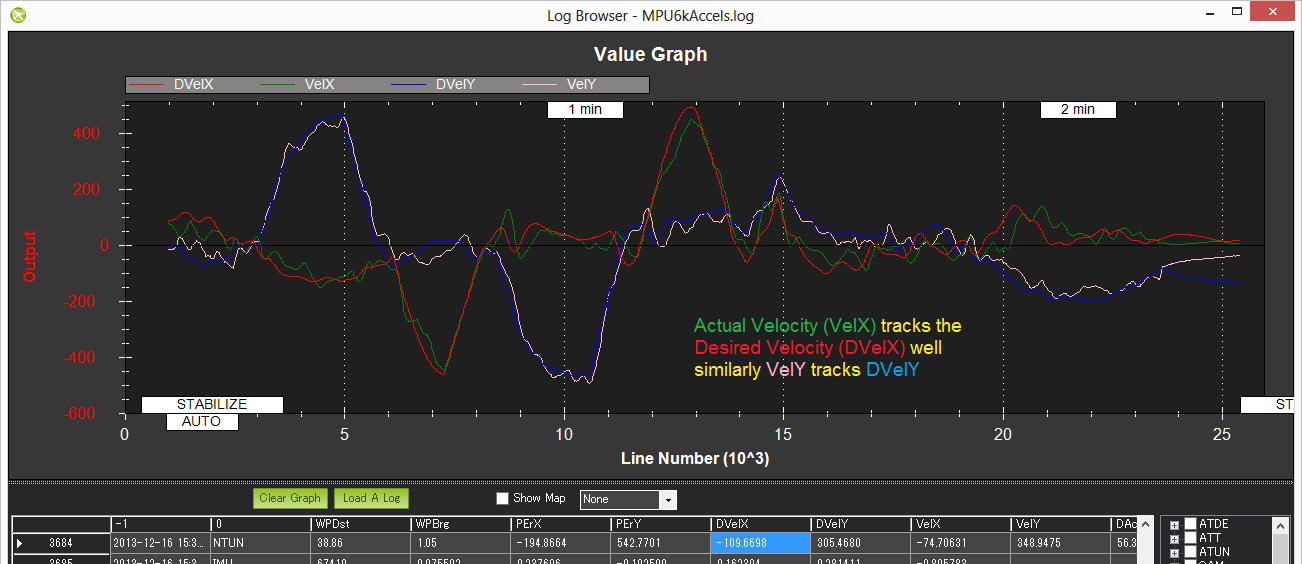
\includegraphics[width=1.0\linewidth]{Loiter_TuningCheck}
	\centering
	\caption{\label{fig: Loiter_TuningCheck}\textit{Loiter Mode Tuning Check using dataflash logs}}
	\end{figure}

\subsection{Verifying performance with dataflash logs}
Viewing the stabilize mode performance is best done by downloading a dataflash log from our flight. We opened it with the mission planner and graph the ATT message’s Roll-In or DesRoll (pilot desired roll angle) vs Roll (actual roll) and Pitch-In or DesPitch (desired pitch angle) vs Pitch (actual pitch angle). These two should track well as shown in Fig.~\ref{fig: Tuning_StabilizeCheck} for our flight test.
\begin{figure}[h]
	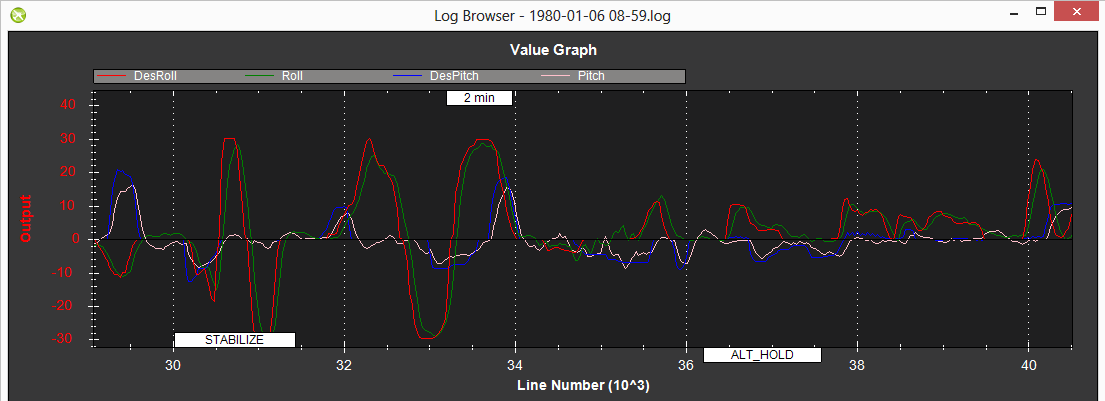
\includegraphics[width=1.0\linewidth]{Tuning_StabilizeCheck}
	\centering
	\caption{\label{fig: Tuning_StabilizeCheck}\textit{Stability Check using dataflash logs}}
\end{figure}

Some flight tests for autonomous flight have been conducted where we achieved the success of flying the flight in the modes mentioned above with considerably great stability. The images of some flight tests are shown in Fig.~\ref{fig: auto_self_I} and Fig.~\ref{fig: auto_self_II}.


\begin{figure}[h]
	\hfill
	\subfigure[]{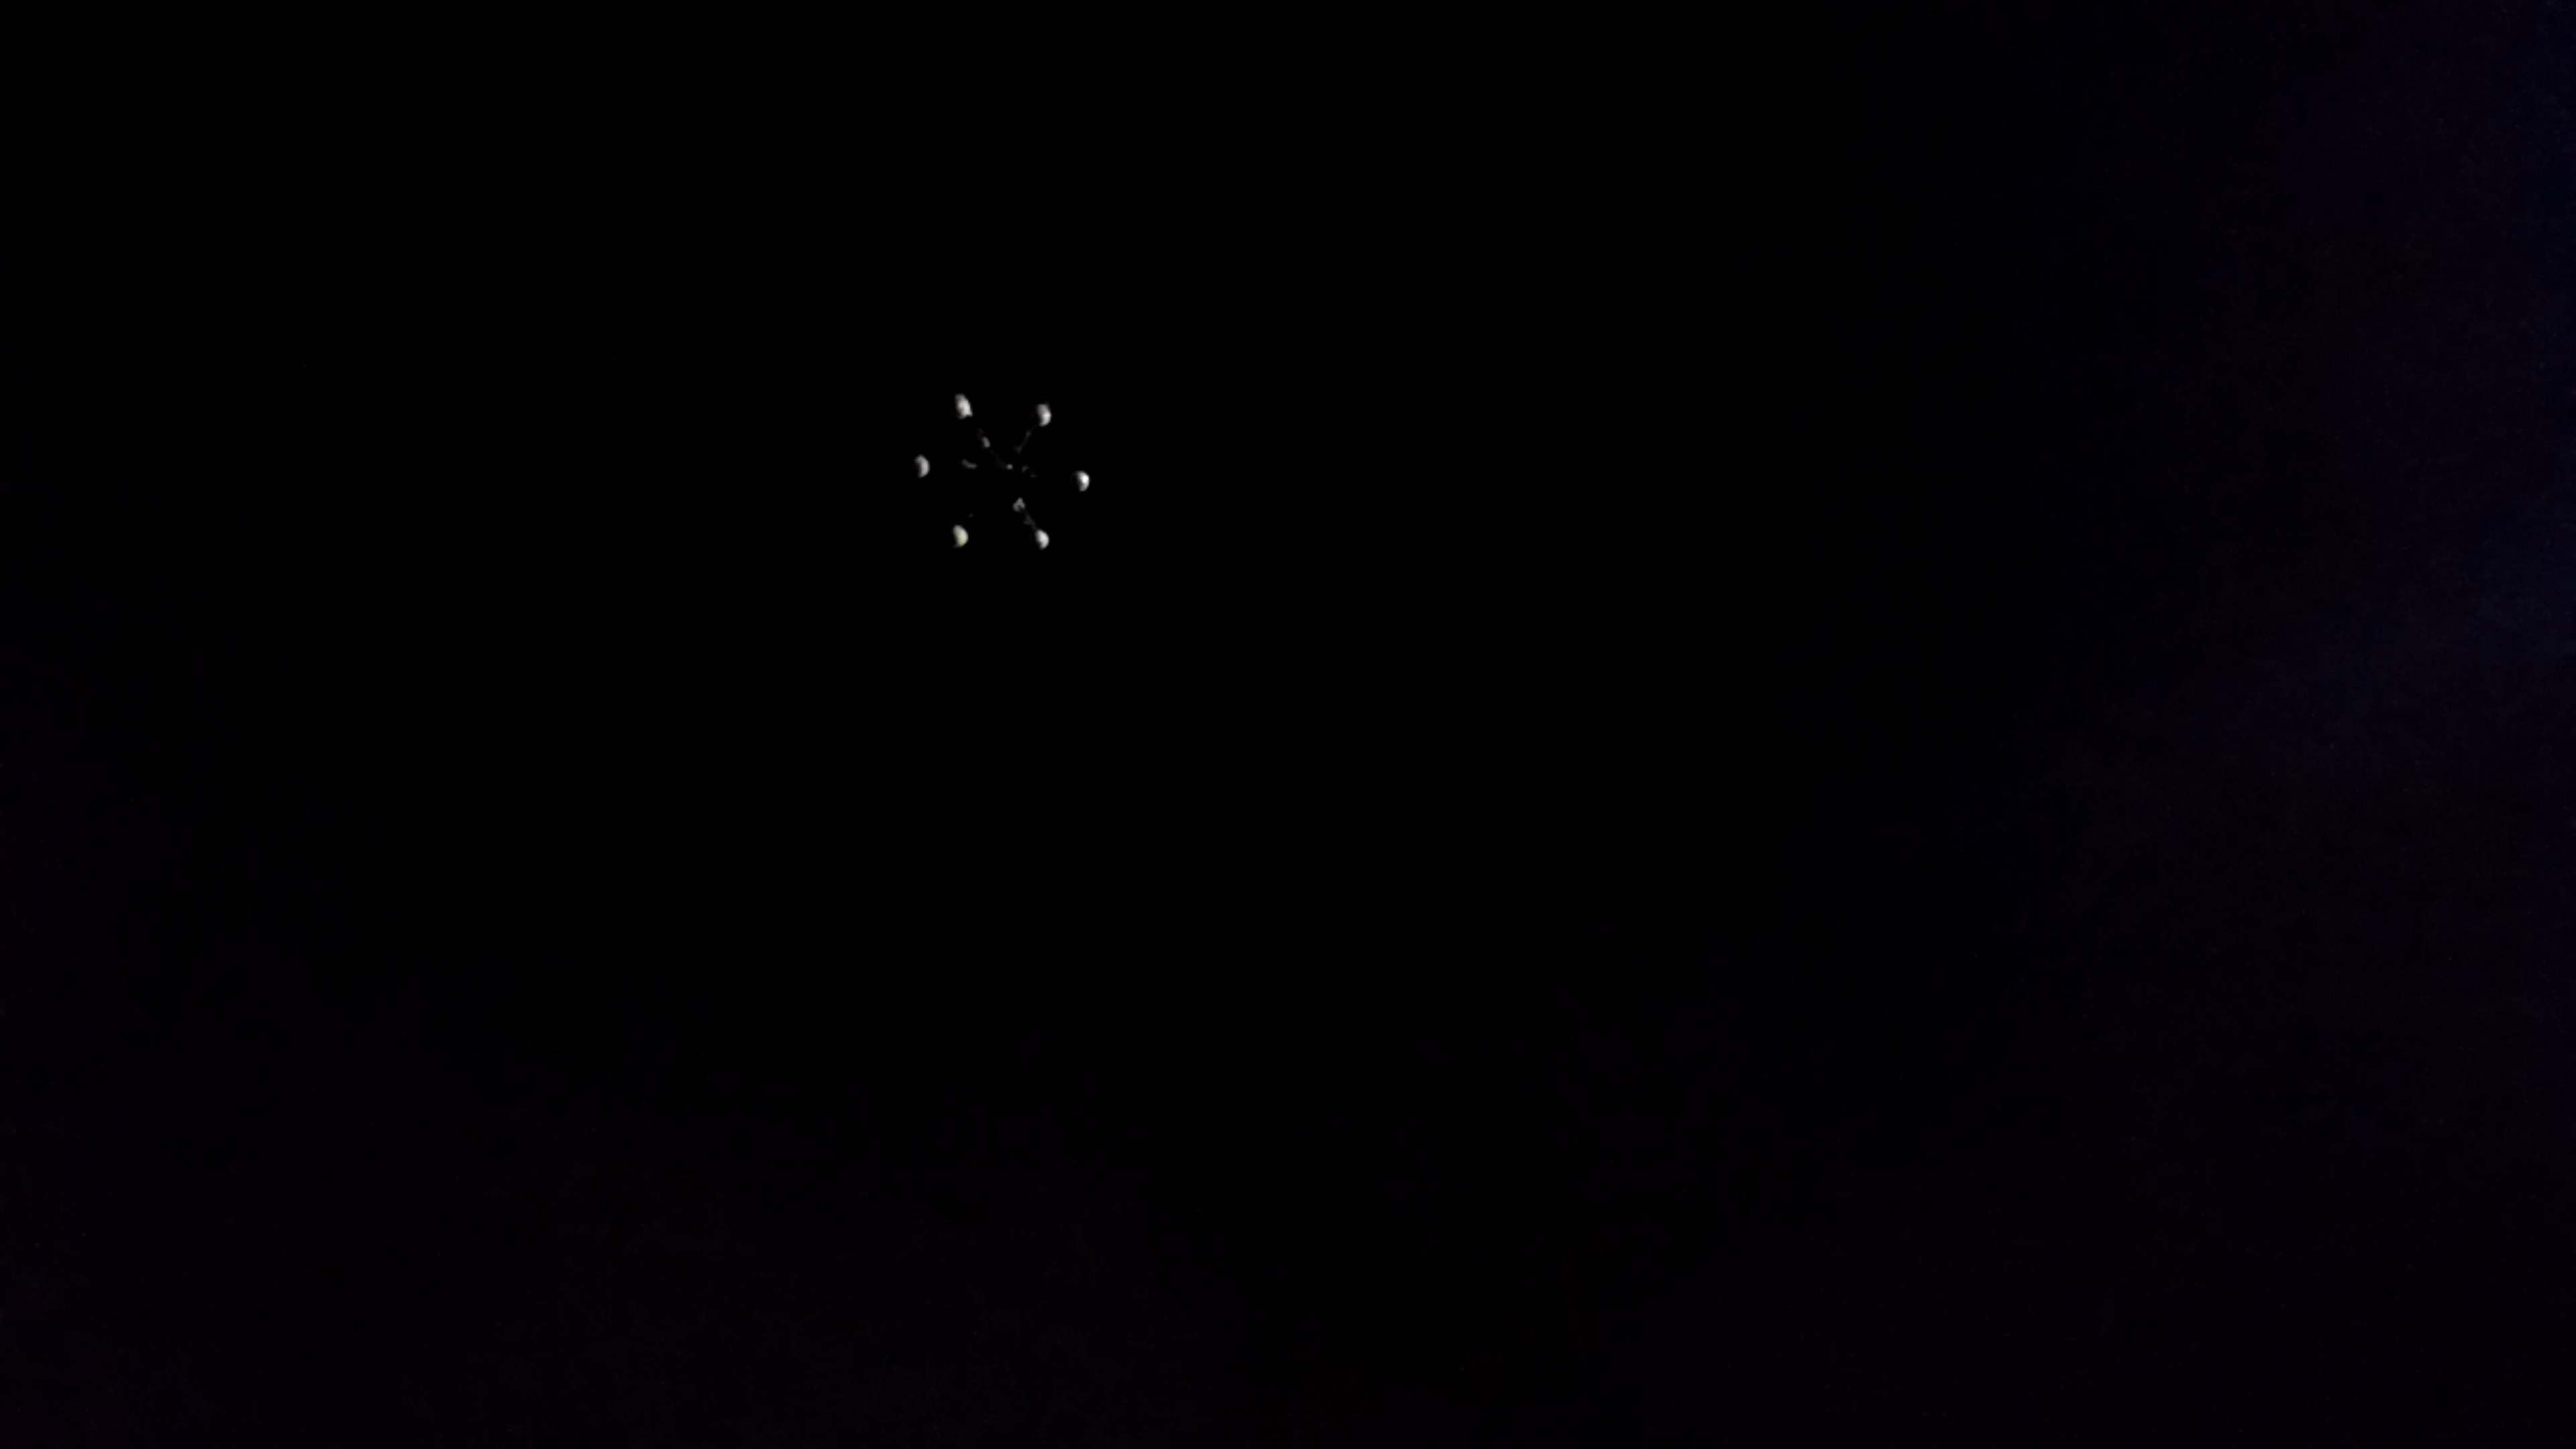
\includegraphics[width=0.48\linewidth]{auto_self_1}}
	\hfill
	\subfigure[]{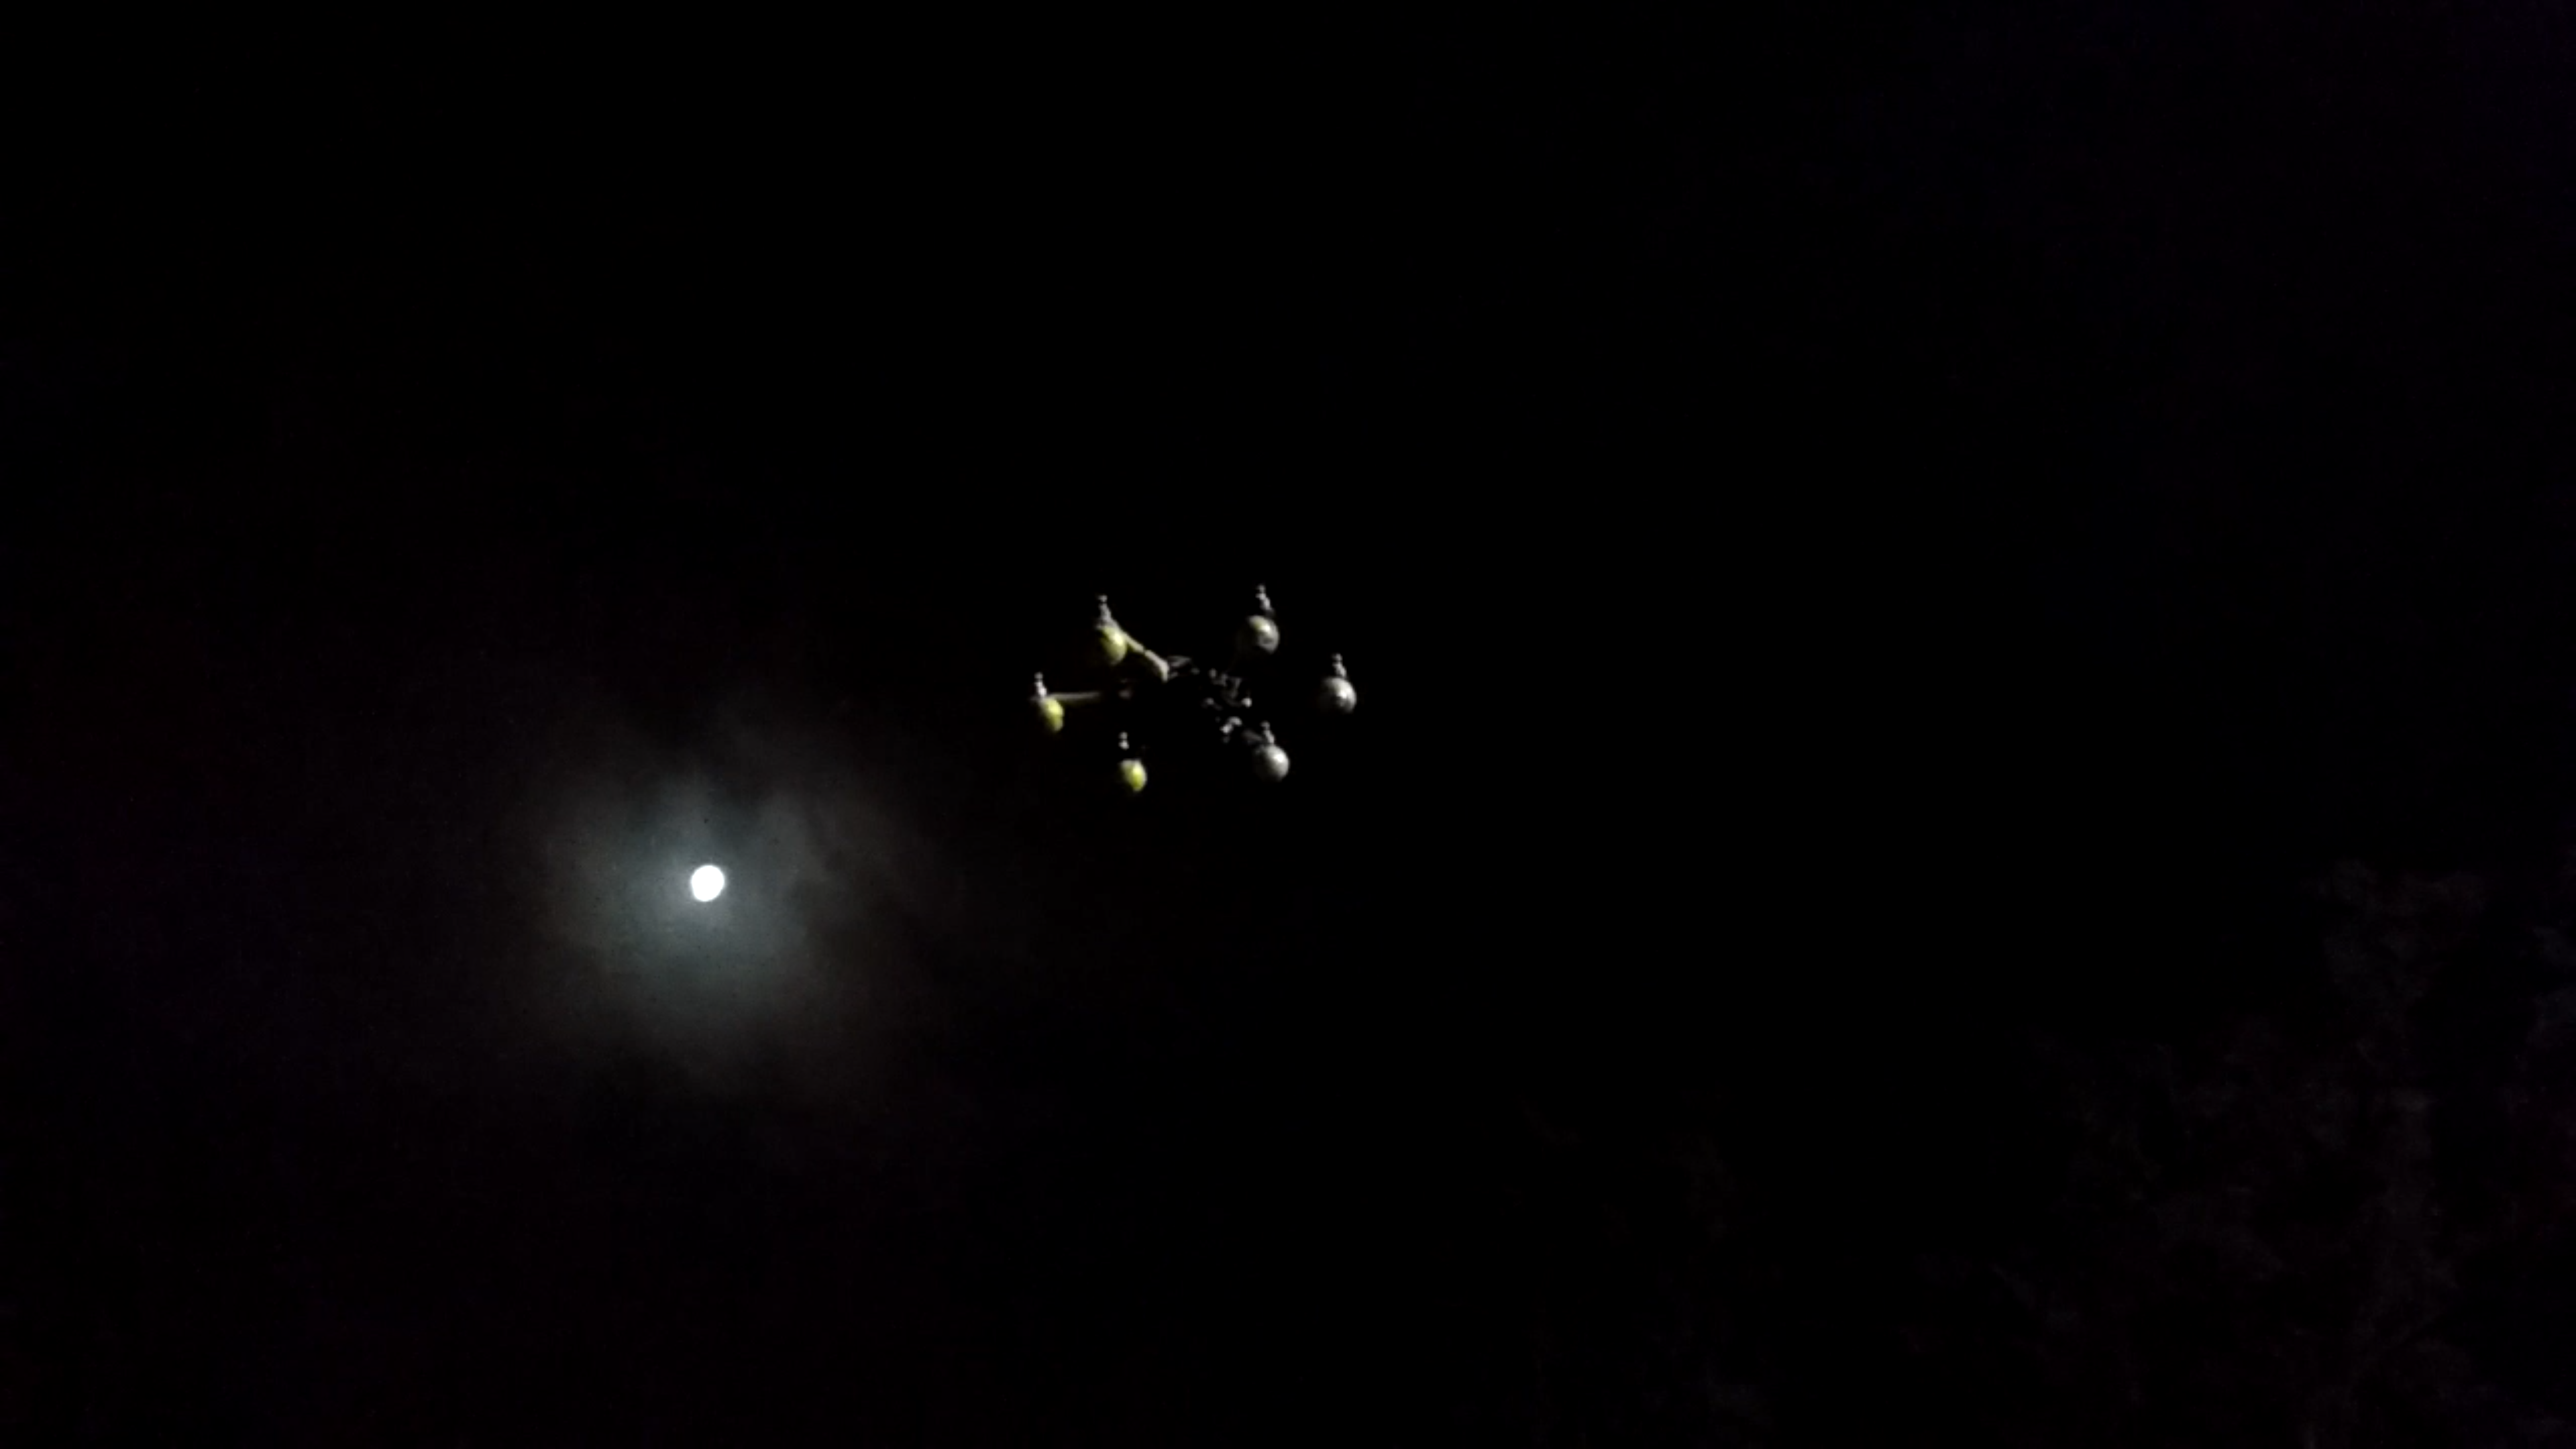
\includegraphics[width=0.48\linewidth]{auto_self_2}}
	\hfill
	\caption{\label{fig: auto_self_I}Flight test data (images) taken during night at Old CRC Lawns in SVNIT Campus}
\end{figure}

\begin{figure}[h]
	\hfill
	\subfigure[]{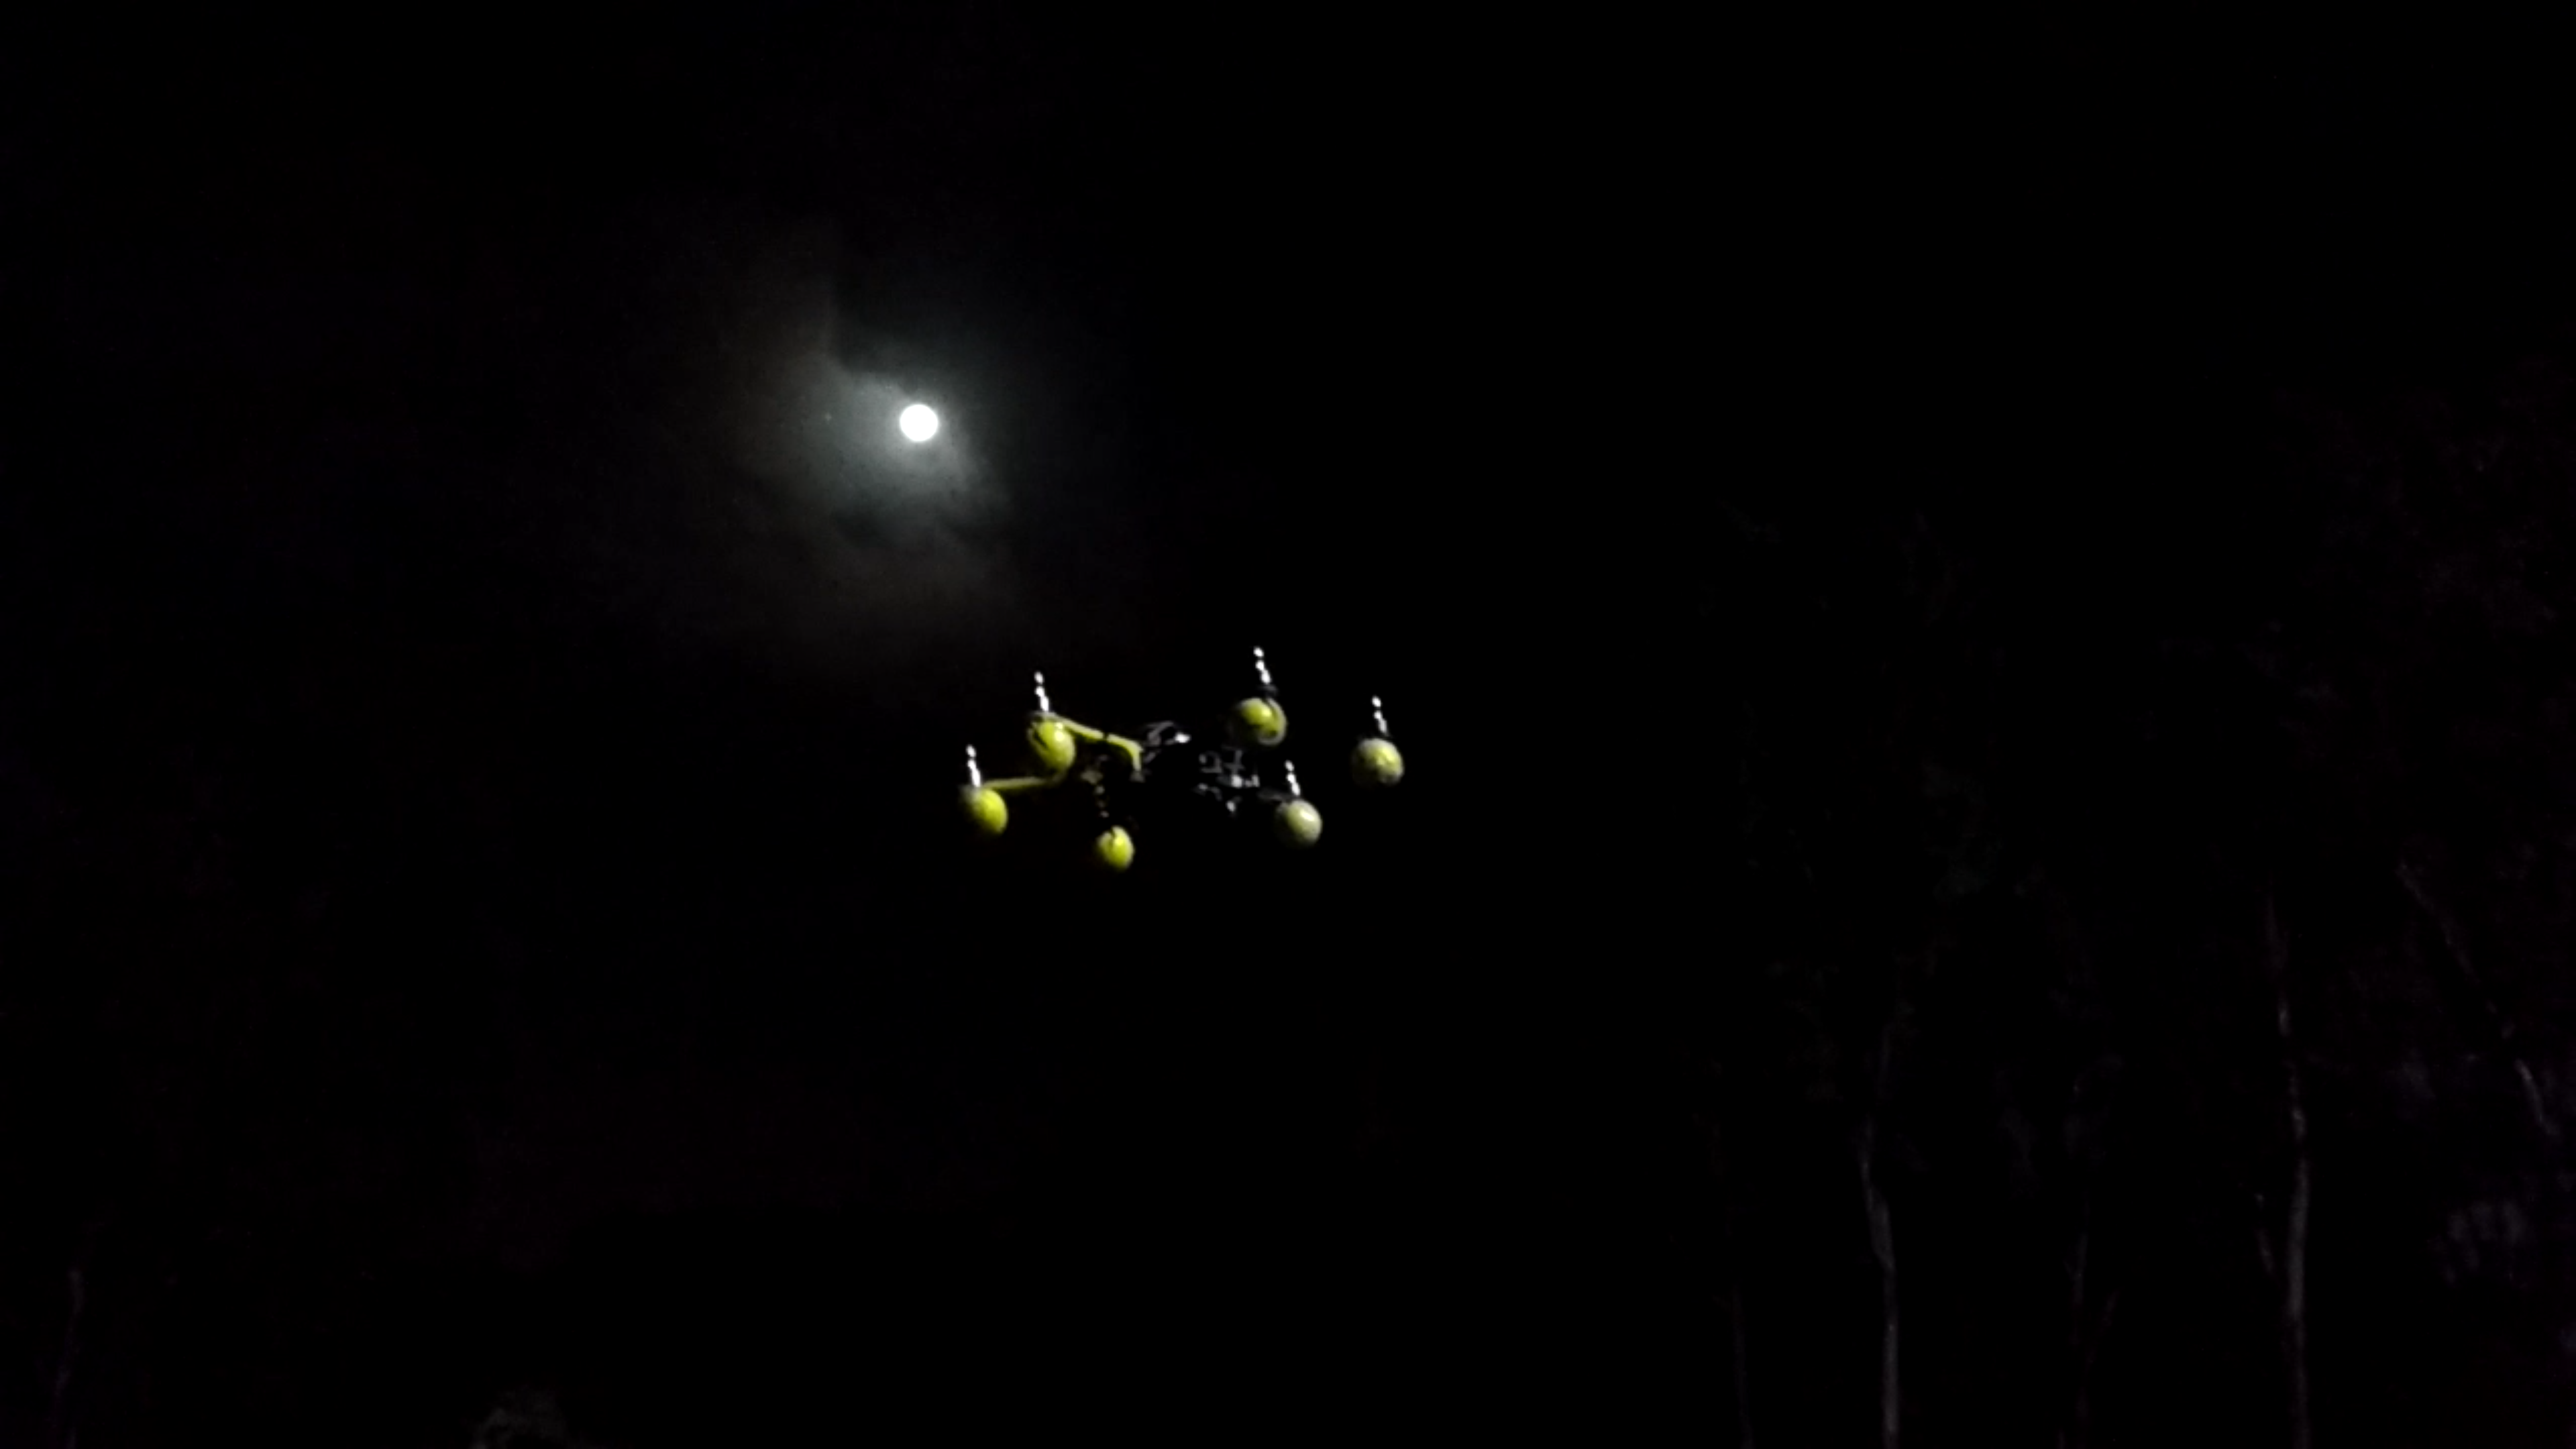
\includegraphics[width=0.48\linewidth]{auto_self_3}}
	\hfill
	\subfigure[]{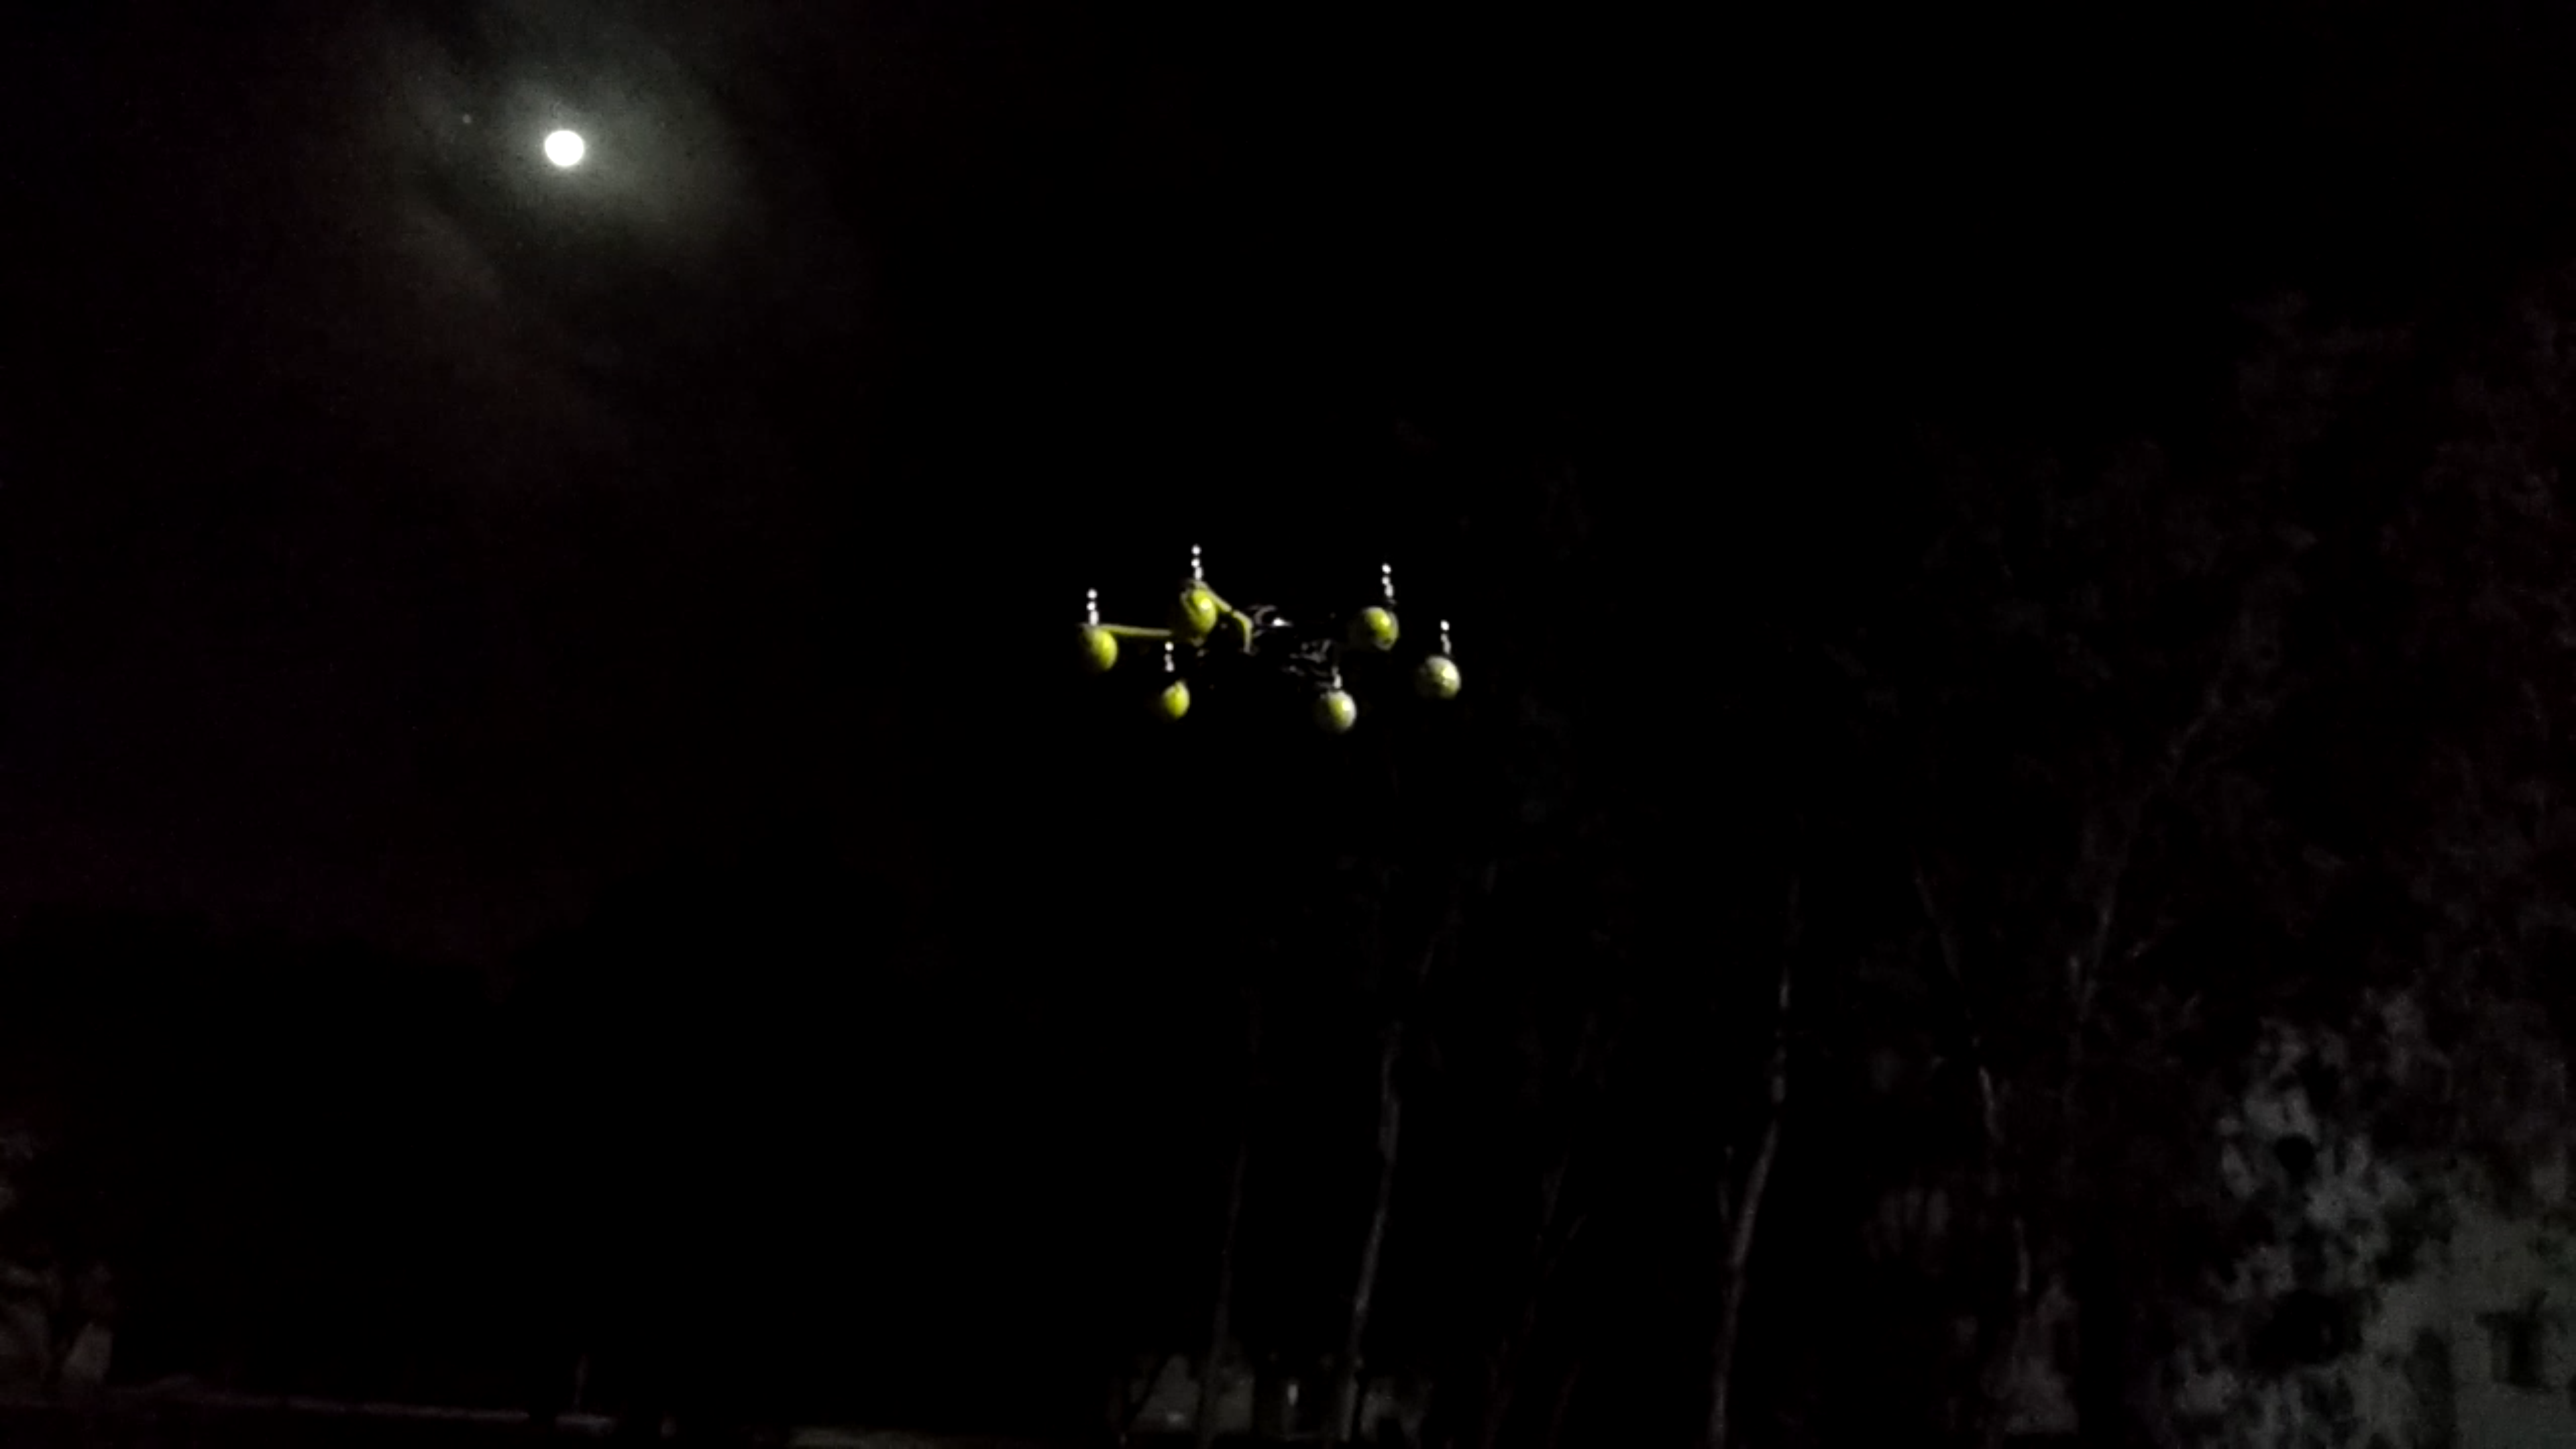
\includegraphics[width=0.48\linewidth]{auto_self_4}}
	\hfill
	\caption{\label{fig: auto_self_II}Flight test data (images) taken during night at Old CRC Lawns in SVNIT Campus}
\end{figure} 


\subsection{Planning a Mission with Waypoints and Events}

Home position, integral to our mission is needed to be set first. For that, the home position is set as the location where the copter was armed. This means if we execute an RTL in Copter, it will return to the location where it was armed, so we armed our copter in the location we wanted it to return to.
\begin{figure}[h]
	\includegraphics[width=1.0\linewidth]{svnit_auto_1}
	\centering
	\caption{\label{fig: svnit_auto_1}\textit{Arming the copter at the Old-CRC Lawns in our S.V.N.I.T. Campus}}
\end{figure}
As we can see in Fig.~\ref{fig: svnit_auto_1}, we initially armed our hex-copter near the Old-CRC lawns area in S.V.N.I.T. Campus. 

Then, as shown in Fig.~\ref{fig: svnit_auto_2}, a Copter mission starts with an auto takeoff to 5 meters attitude; then goes to WP 1, then waits 10 seconds; then the craft will proceed to WP 2 followed by WP 3, then returns to launch. After reaching the launch position, the craft will land. The mission assumes that the launch position is set at the home position.

\begin{figure}[h]
	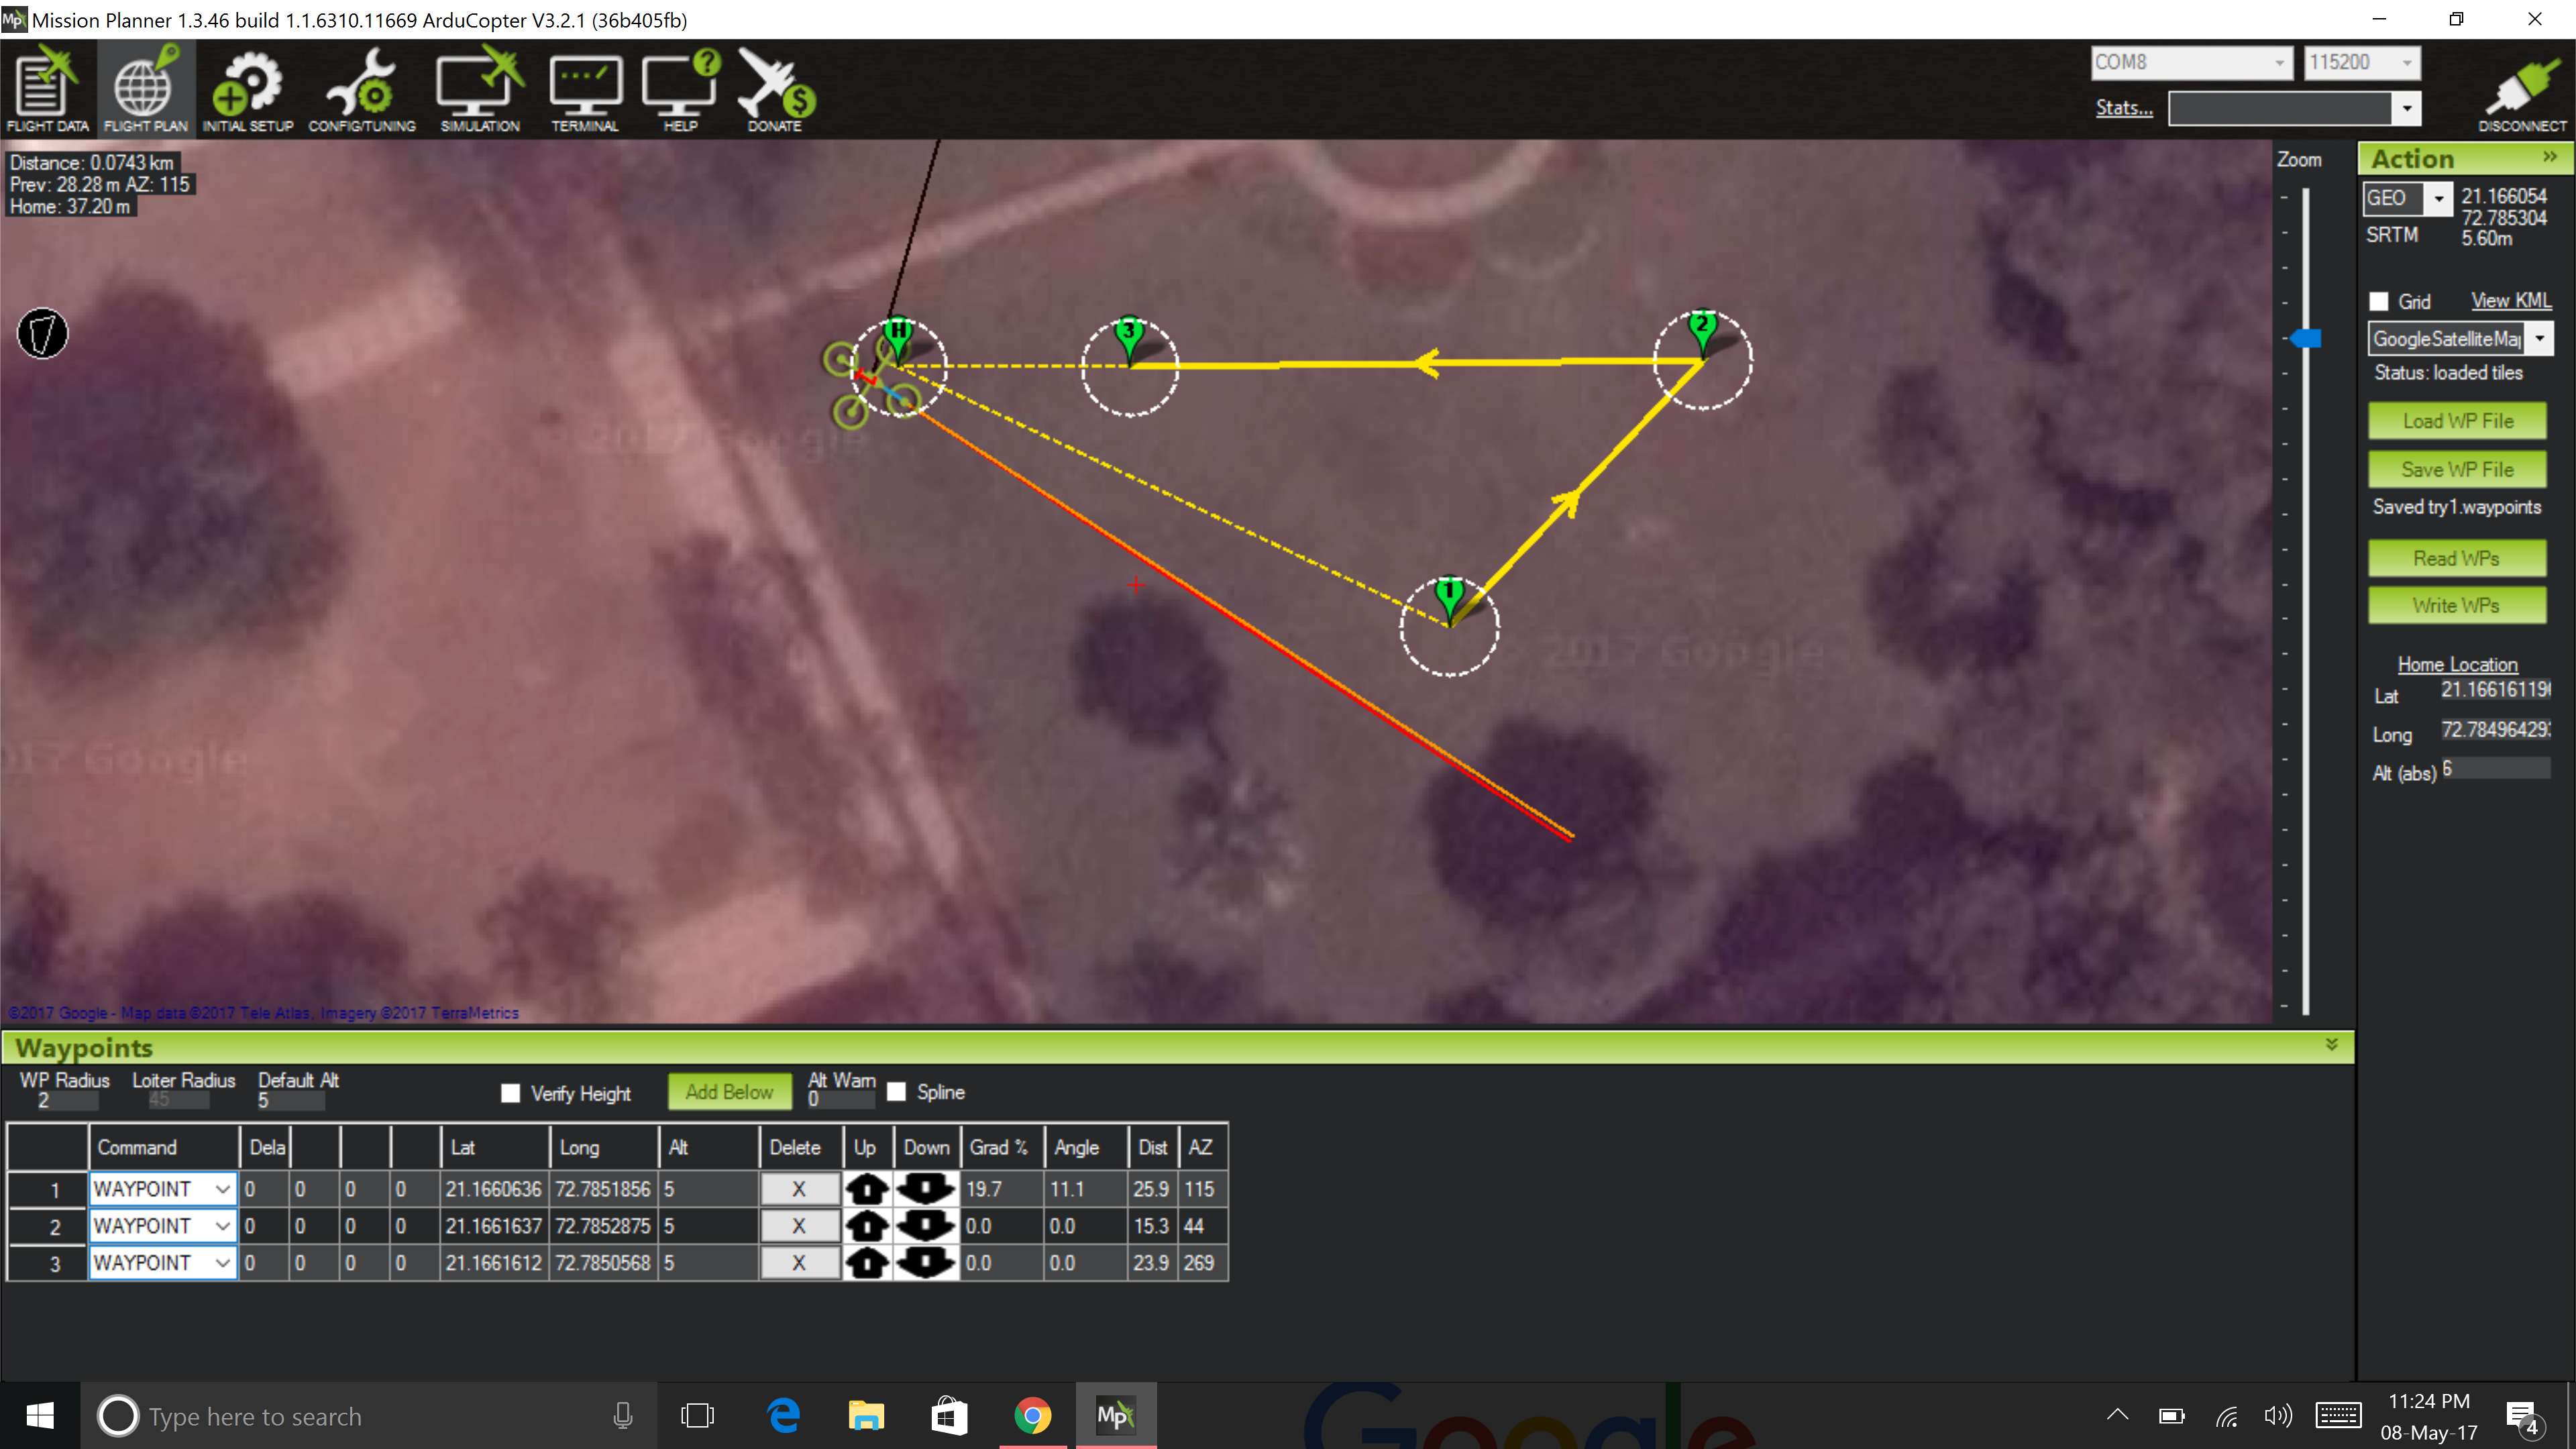
\includegraphics[width=1.0\linewidth]{svnit_auto_2}
	\centering
	\caption{\label{fig: svnit_auto_2}\textit{Planning a mission at CRC Lawns}}
\end{figure}

We can enter waypoints and other commands (see the Mission commands section below for more information). In the dropdown menus on each row, we can select the command we want. The column heading will change to show us what data that command requires. Lat and Lon can be entered by clicking on the map. Altitude is relative to our launch altitude/home position.

Once we are done with our mission, we would select Write and it will be sent to APM and saved in EEPROM. We can confirm that it’s as we wanted by selecting Read.

We can save multiple mission files to your local hard drive by selecting Save WP File or read in files with Load WP File in the right-click menu. 

\subsection{Auto grid}

To do something on the terms of precision farming needs, we know that we need our copter to fly a predetermined path obtained through GPS and survey/take available data of crops along the way. For this need, we can set such pattern in Auto grid. So we can have the Mission Planner create a mission for us, which is useful for function like mapping missions, where the aircraft should just go back and forth in a “lawnmower” pattern over an area to collect photographs (say in an agricultural field)


To do this, in the right-click menu we select Polygon and draw a box around the area you want to map. Then we select Auto WP, Grid. We then follow the dialog box process to select altitude and spacing. The Mission Planner will then generate a mission that looks something like this:
\begin{figure}[h]
	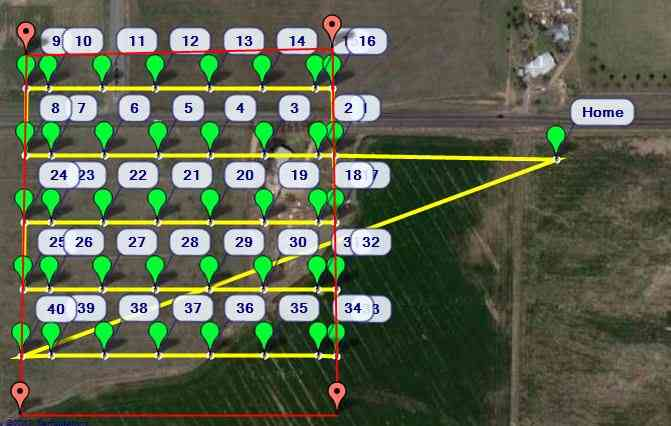
\includegraphics[width=1.0\linewidth]{mp_auto_mission_grid}
	\centering
	\caption{\label{fig: mp_auto_mission_grid}\textit{Mission pertaining to our need for precision farming application}}
\end{figure}



Below given is the detailed specification of autonomous flight accomplished in the SAC Ground, S.V.N.I.T. Campus, Surat, Gujarat, India. 

\begin{figure}[h]
	\hfill
	\subfigure[]{\includegraphics[width=0.48\linewidth]{finmis1}}
	\hfill
	\subfigure[]{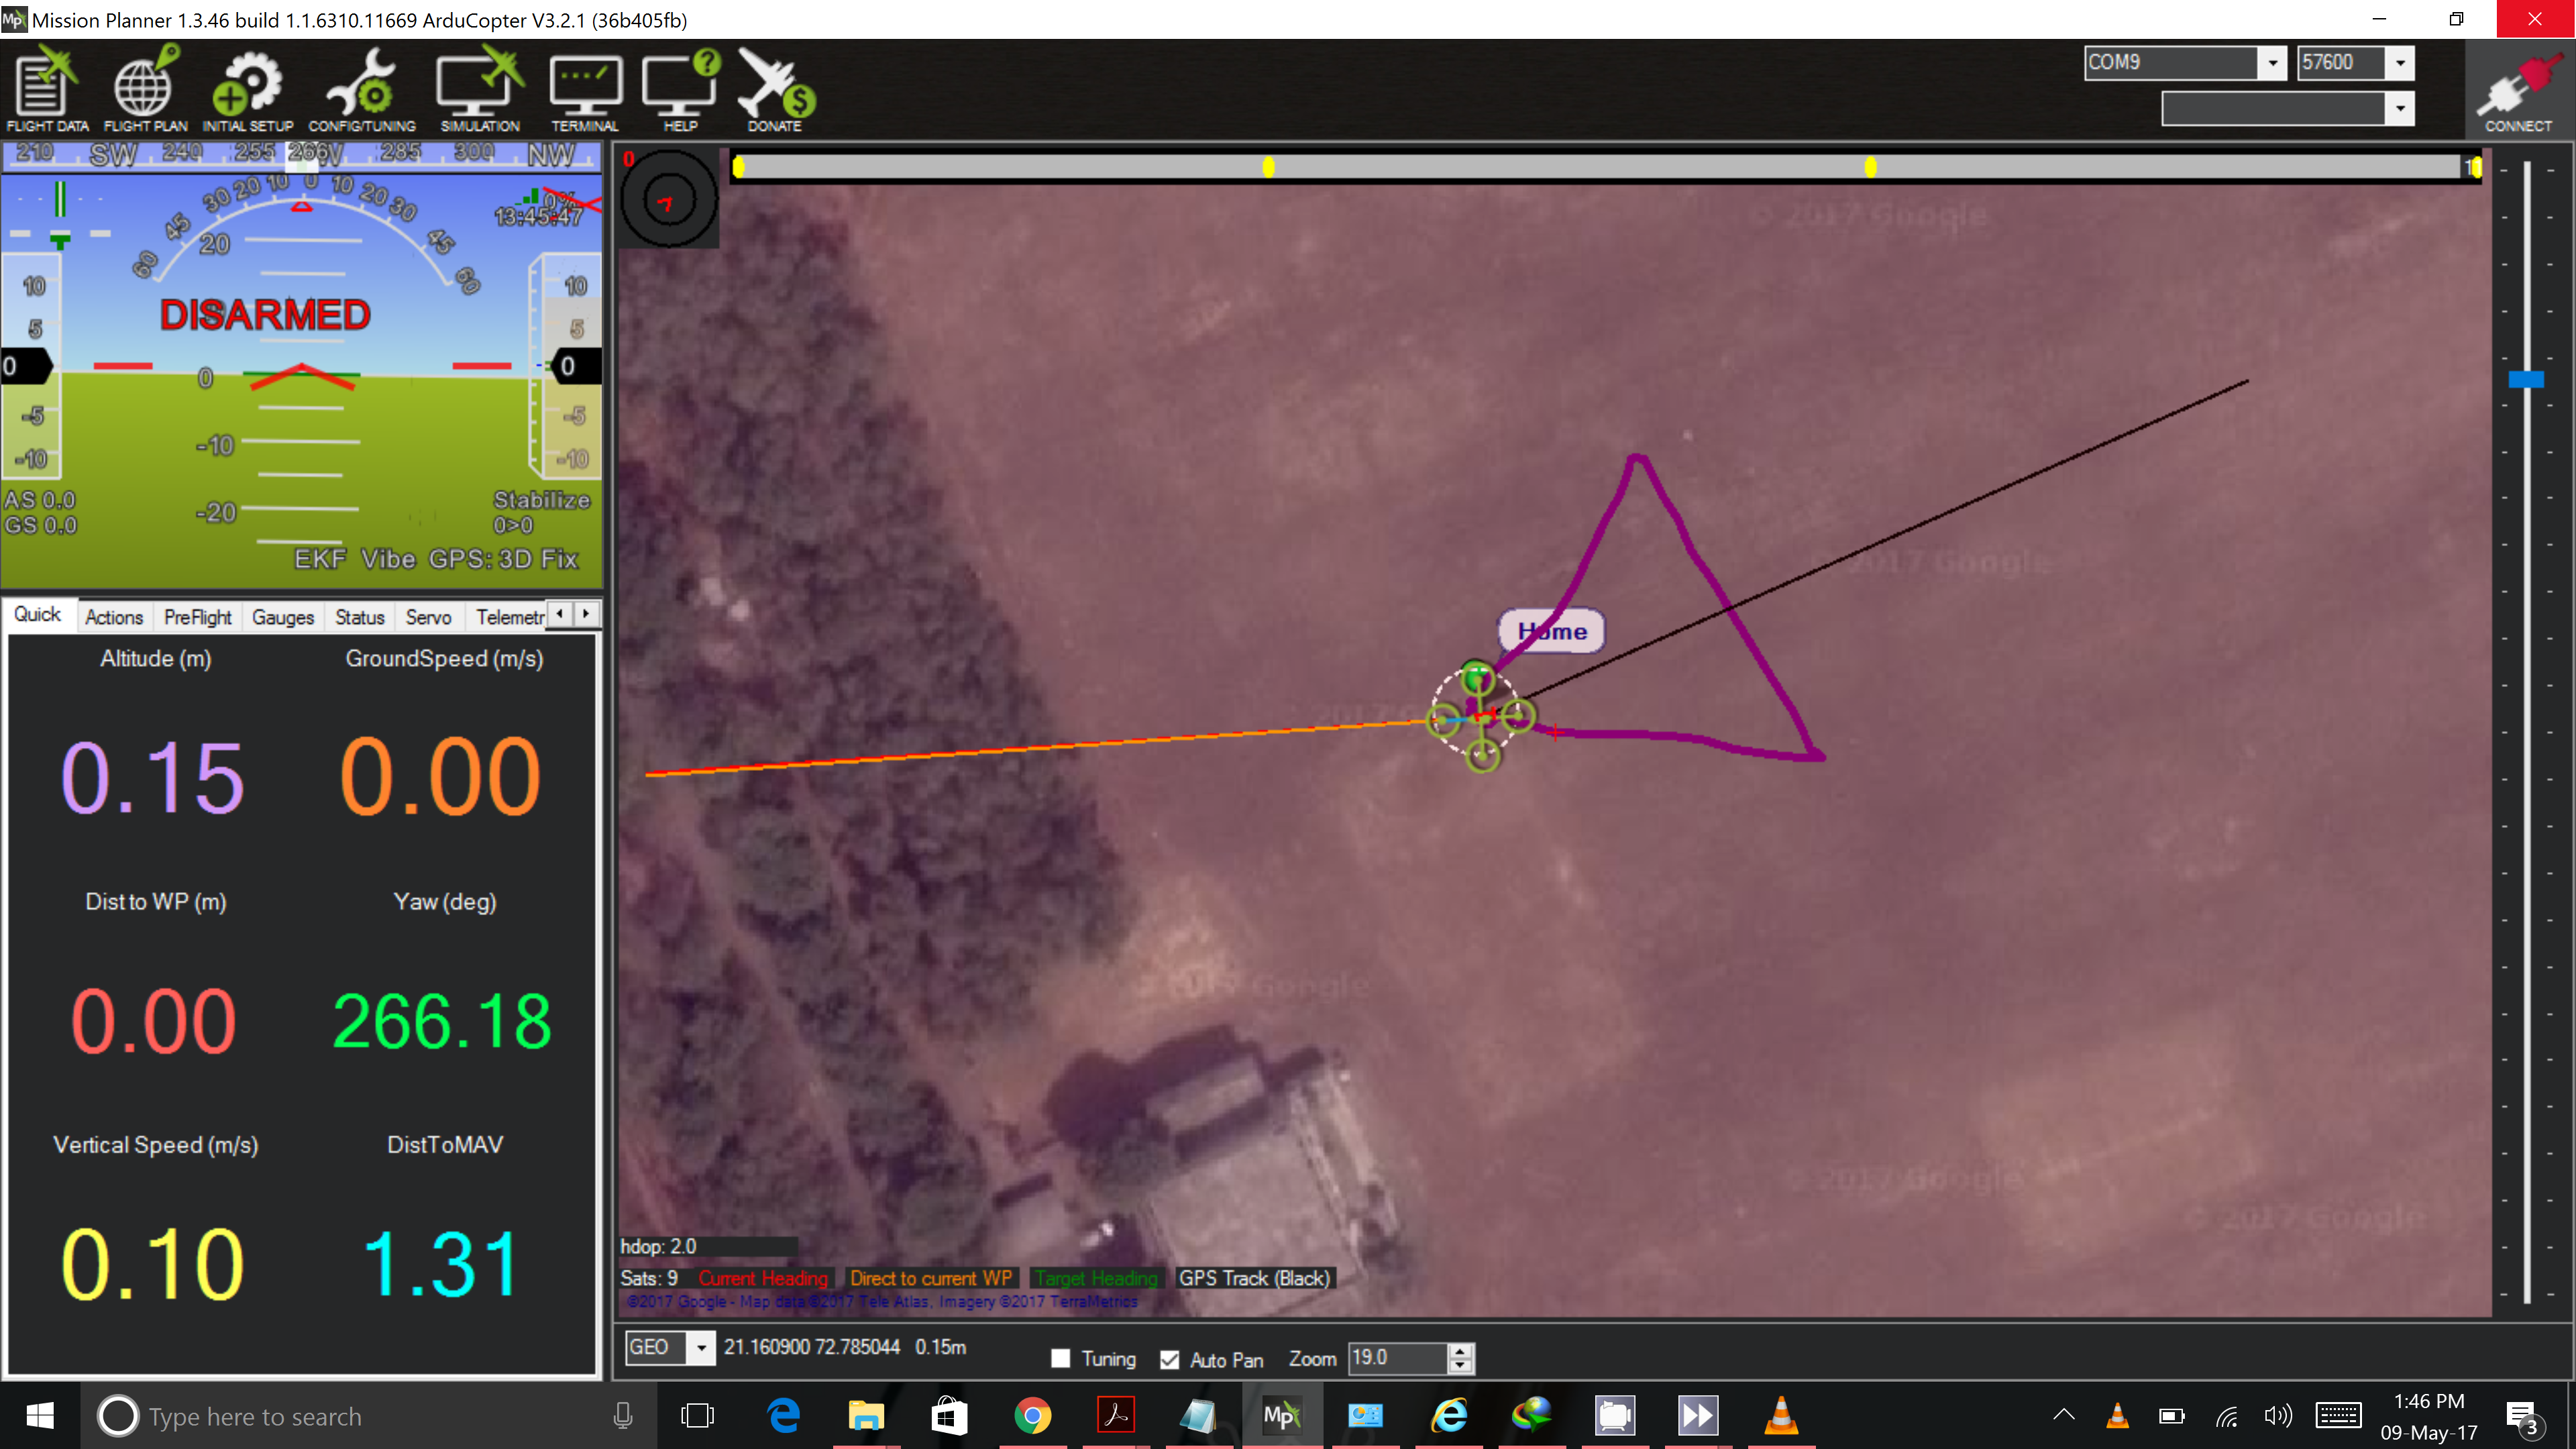
\includegraphics[width=0.48\linewidth]{finmis2}}
	\hfill
	\caption{\label{fig: fin_mis}Fig.(a) shows the desired path given by the user. Fig.(b) shows the actual traced trajectory in the autonomous mode by the hex-copter.}
\end{figure} 

Fig.~\ref{fig: fin_mis}(a) is showing the desired the path given by the GPS coordinates while Fig.~\ref{fig: fin_mis}(b) shows the actual traced trajectory by the hex-copter.

The screenshots of the autonomous flight are displayed in Fig.~\ref{fig: fin_mis_1}, Fig.~\ref{fig: fin_mis_2}, Fig.~\ref{fig: fin_mis_3} and Fig.~\ref{fig: fin_mis_4}.

\begin{figure}[!h]
	\hfill
	\subfigure[]{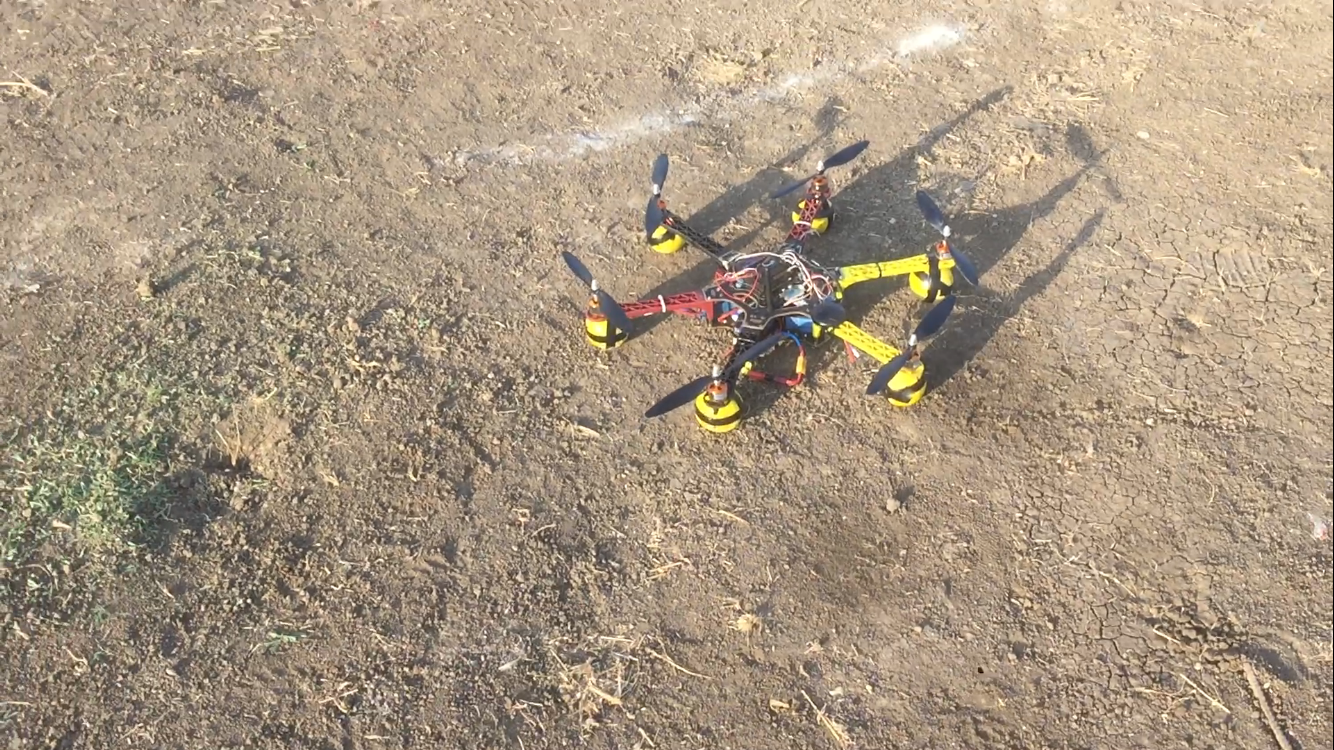
\includegraphics[width=0.48\linewidth]{finmis_1}}
	\hfill
	\subfigure[]{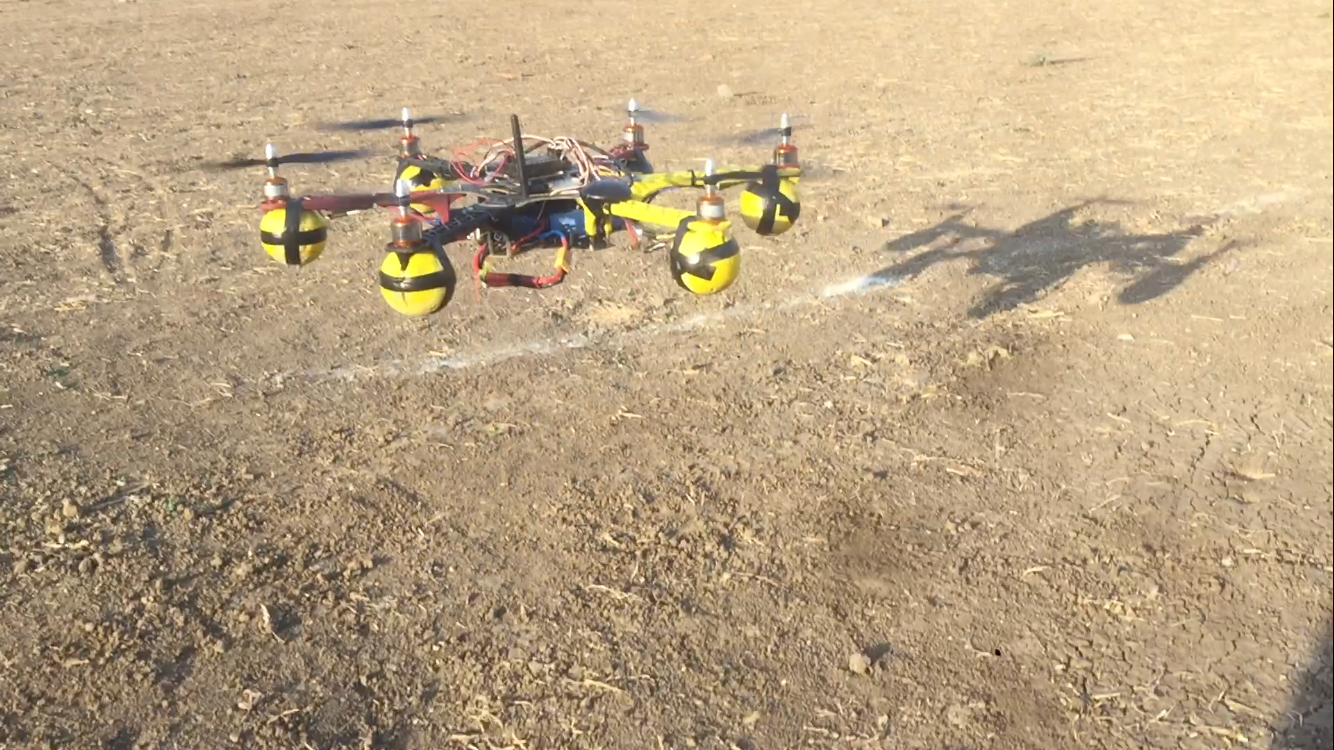
\includegraphics[width=0.48\linewidth]{finmis_2}}
	\hfill
	\caption{\label{fig: fin_mis_1}Different modes, including takeoff, hover and going to waypoints are shown above}
\end{figure} 


\begin{figure}[!h]
	\hfill
	\subfigure[]{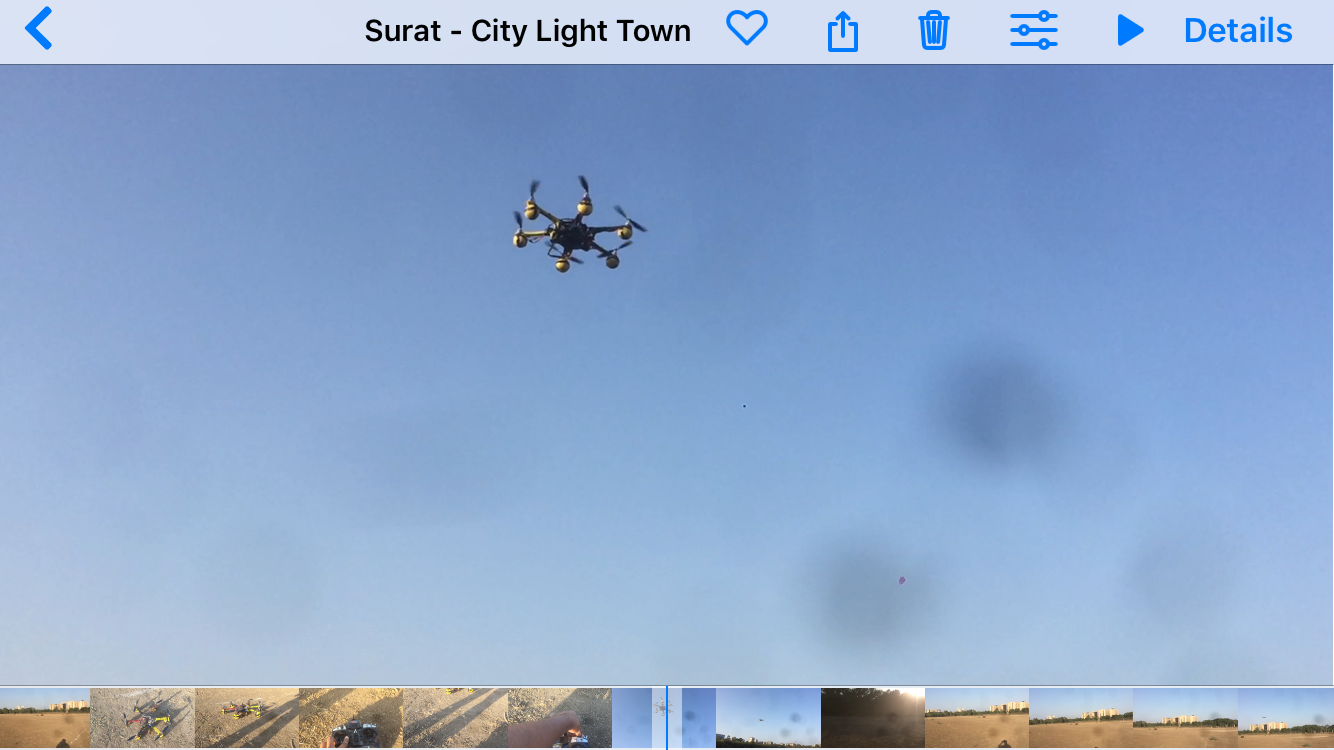
\includegraphics[width=0.48\linewidth]{finmis_3}}
	\hfill
	\subfigure[]{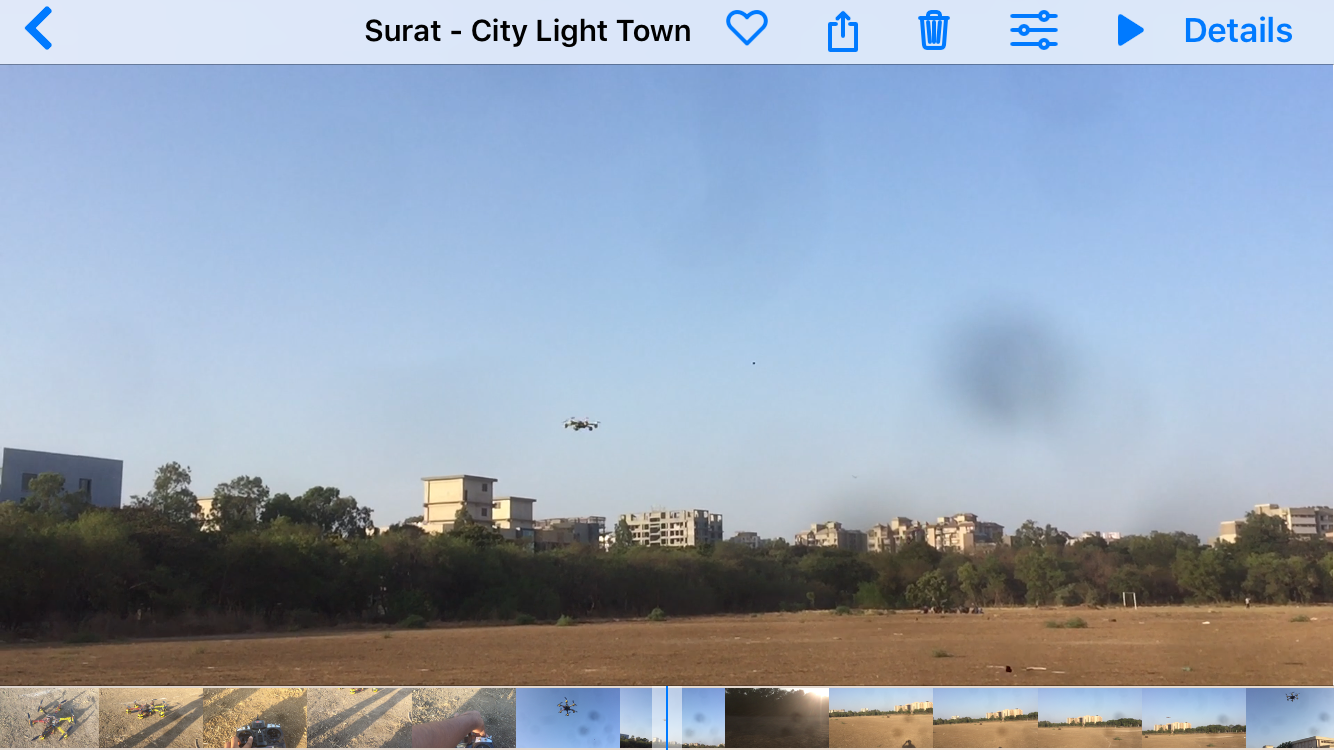
\includegraphics[width=0.48\linewidth]{finmis_4}}
	\hfill
	\caption{\label{fig: fin_mis_2}Different modes, including takeoff, hover and going to waypoints are shown above}
\end{figure} 


\begin{figure}[!h]
	\hfill
	\subfigure[]{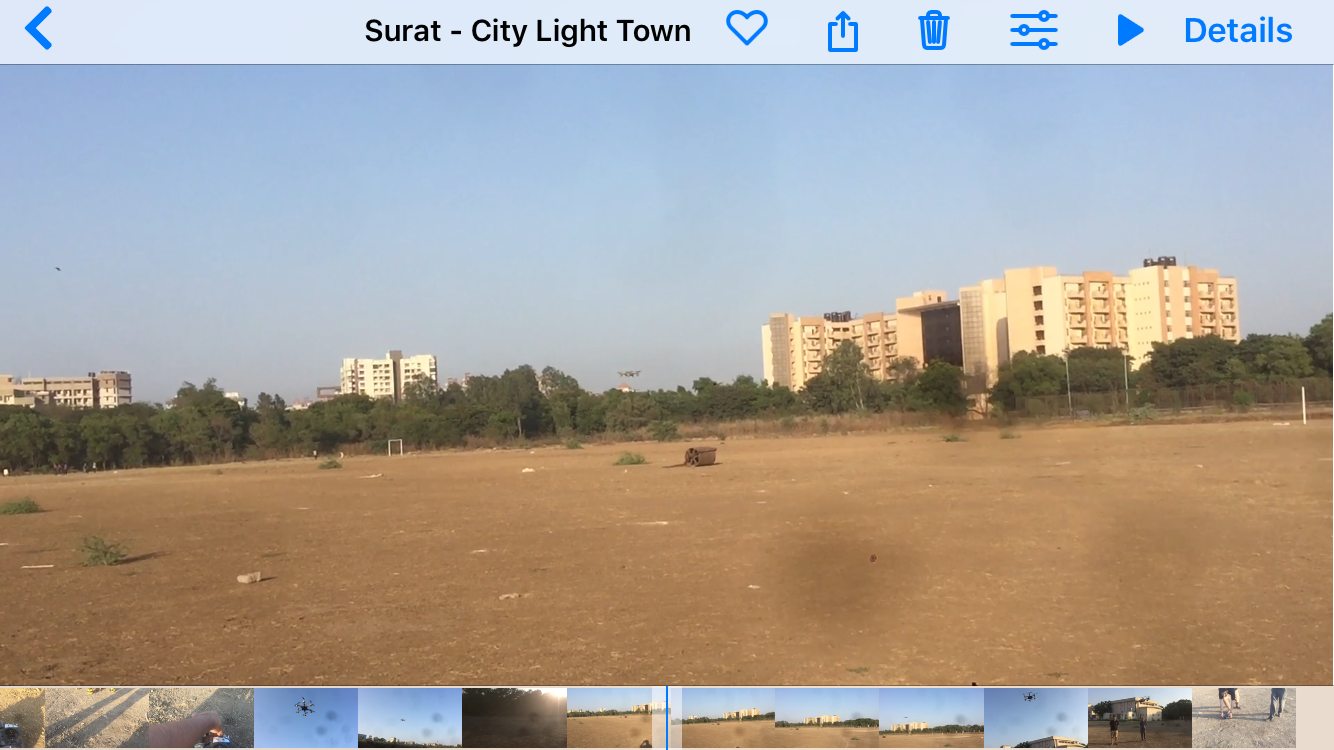
\includegraphics[width=0.48\linewidth]{finmis_5}}
	\hfill
	\subfigure[]{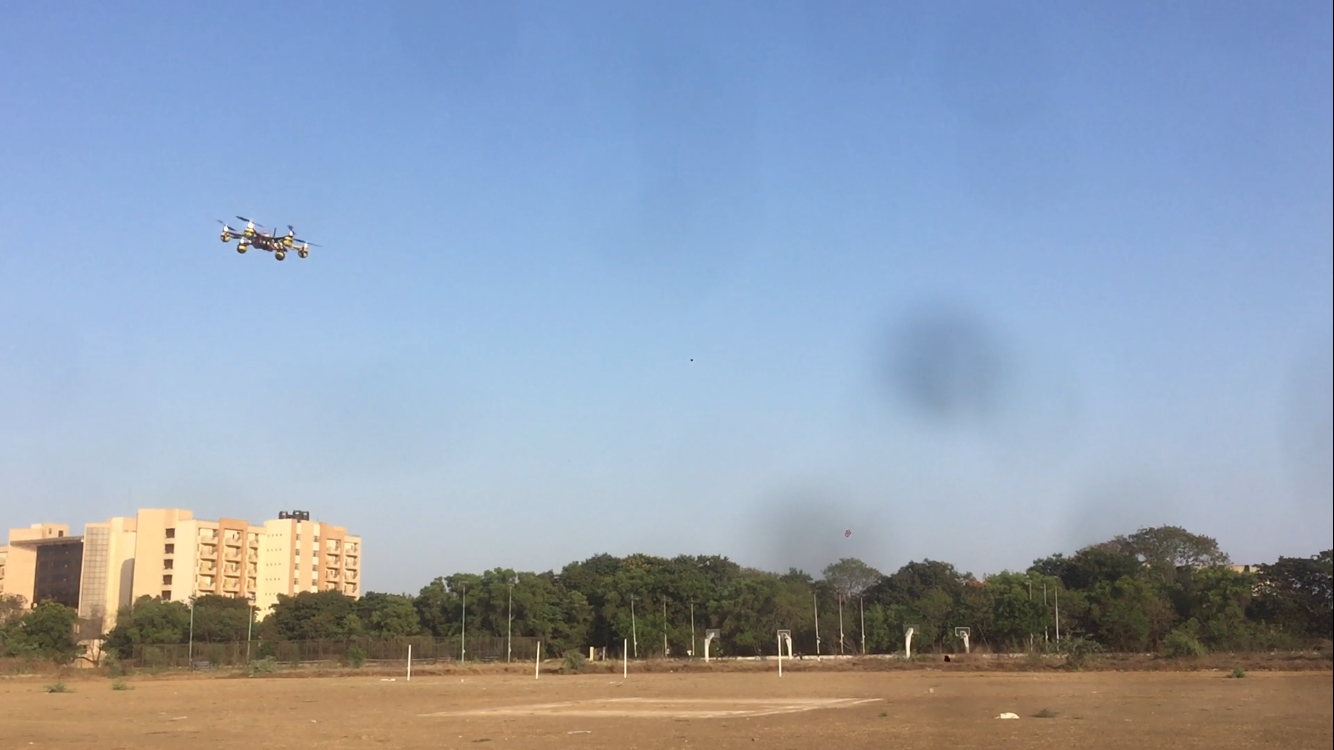
\includegraphics[width=0.48\linewidth]{finmis_6}}
	\hfill
	\caption{\label{fig: fin_mis_3}Different modes, including takeoff, hover and going to waypoints are shown above}
\end{figure} 


\begin{figure}[!h]
	\hfill
	\subfigure[]{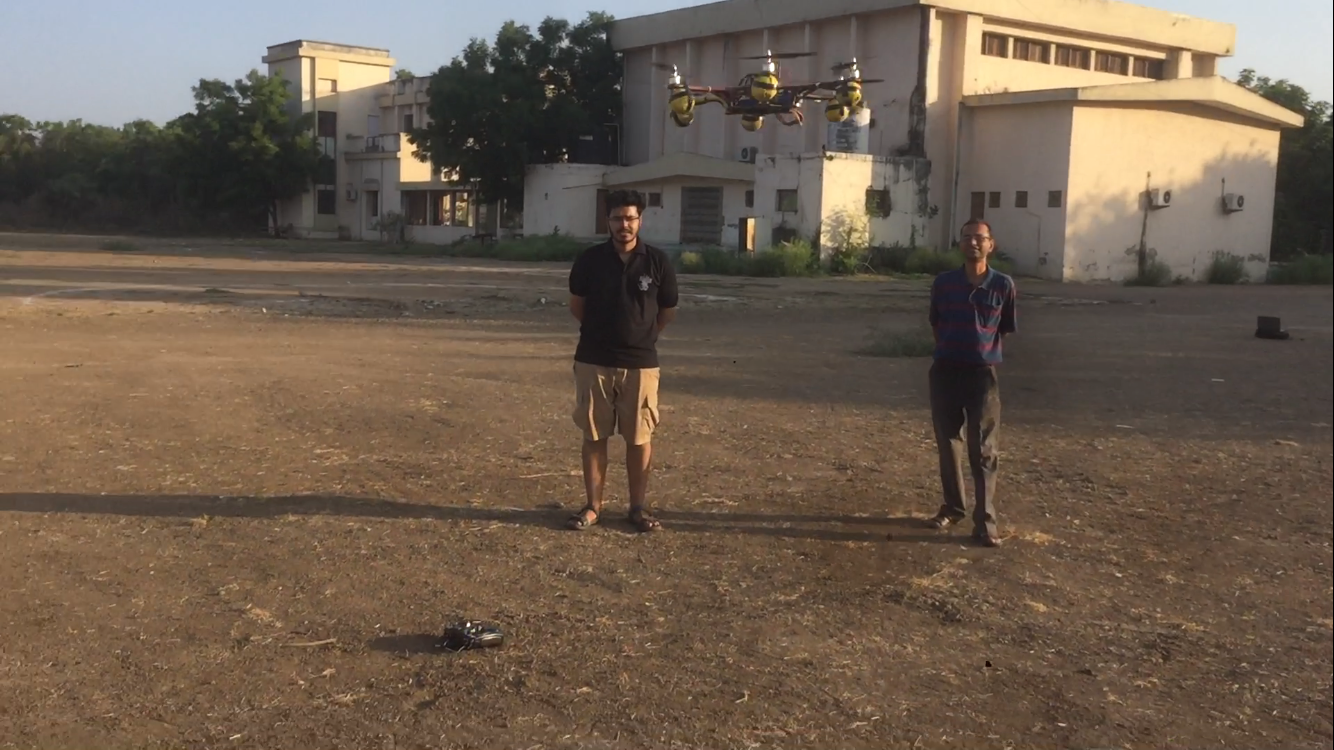
\includegraphics[width=0.48\linewidth]{finmis_7}}
	\hfill
	\subfigure[]{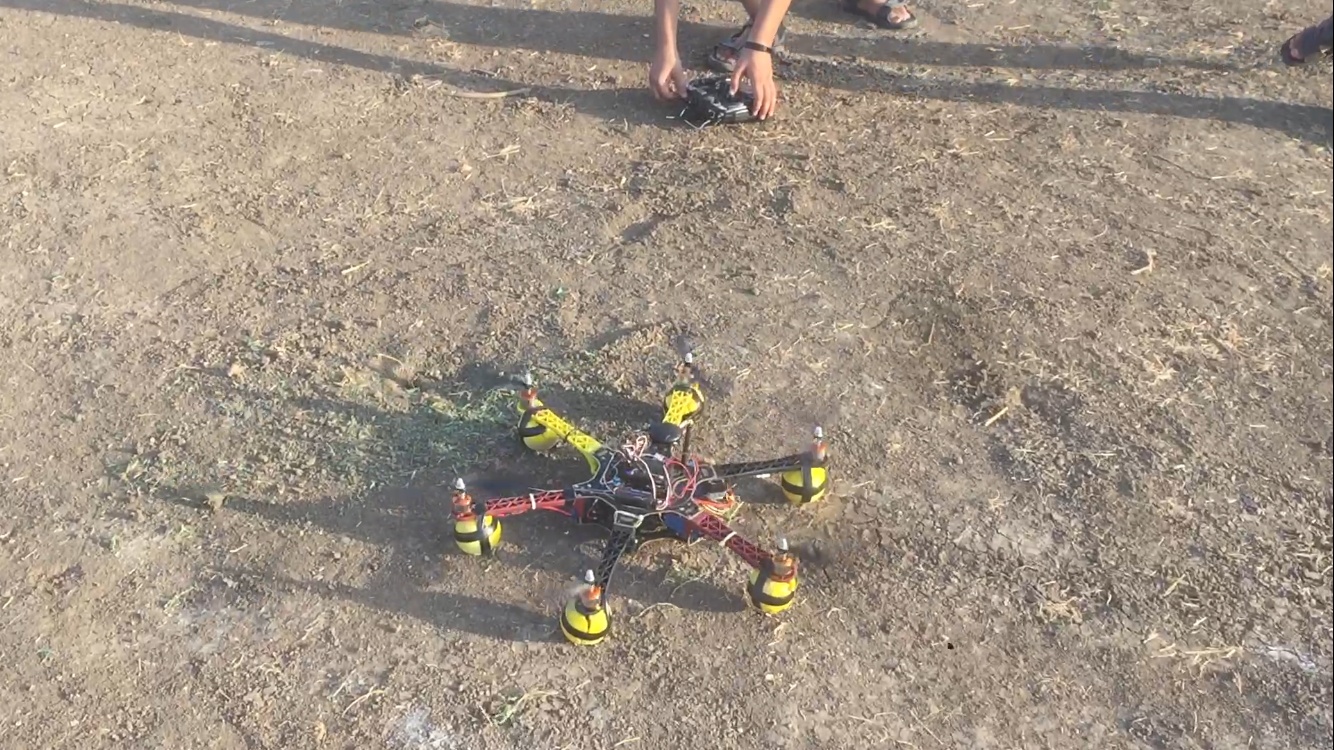
\includegraphics[width=0.48\linewidth]{finmis_8}}
	\hfill
	\caption{\label{fig: fin_mis_4}Different modes, including takeoff, hover and going to waypoints are shown above}
\end{figure} 



\section{Web Portal}

A web portal is built to facilitate the process of farm crop analysis. Web portal provides the functionality of uploading drone images for stitching process. Screenshots of the application portal are shown in Fig.~\ref{fig: web_p}, Fig.~\ref{fig: res-1} and Fig.~\ref{fig: res-2}.



\begin{figure}[h]
	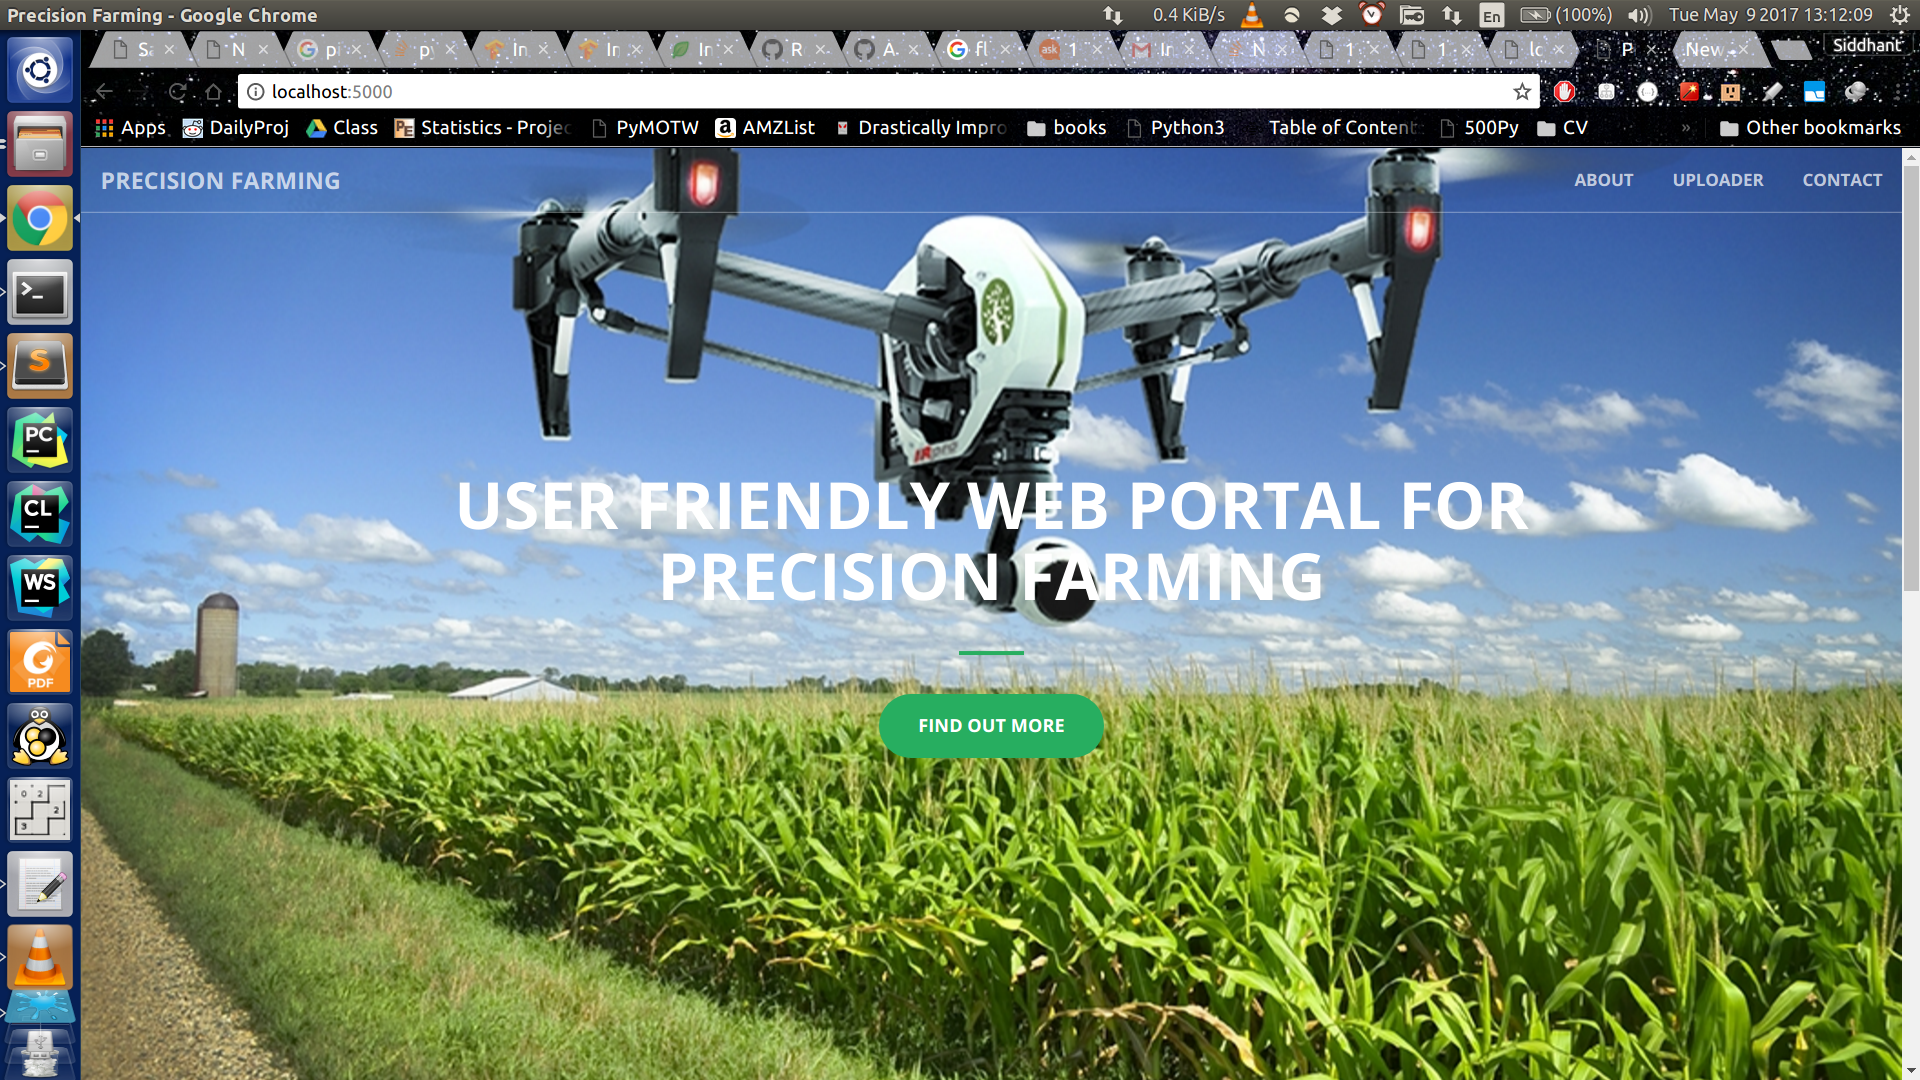
\includegraphics[width=1\linewidth]{webhost_precision}
	\centering
	\caption{\label{fig: web_p}Web portal}
\end{figure}
\begin{figure}[h]
	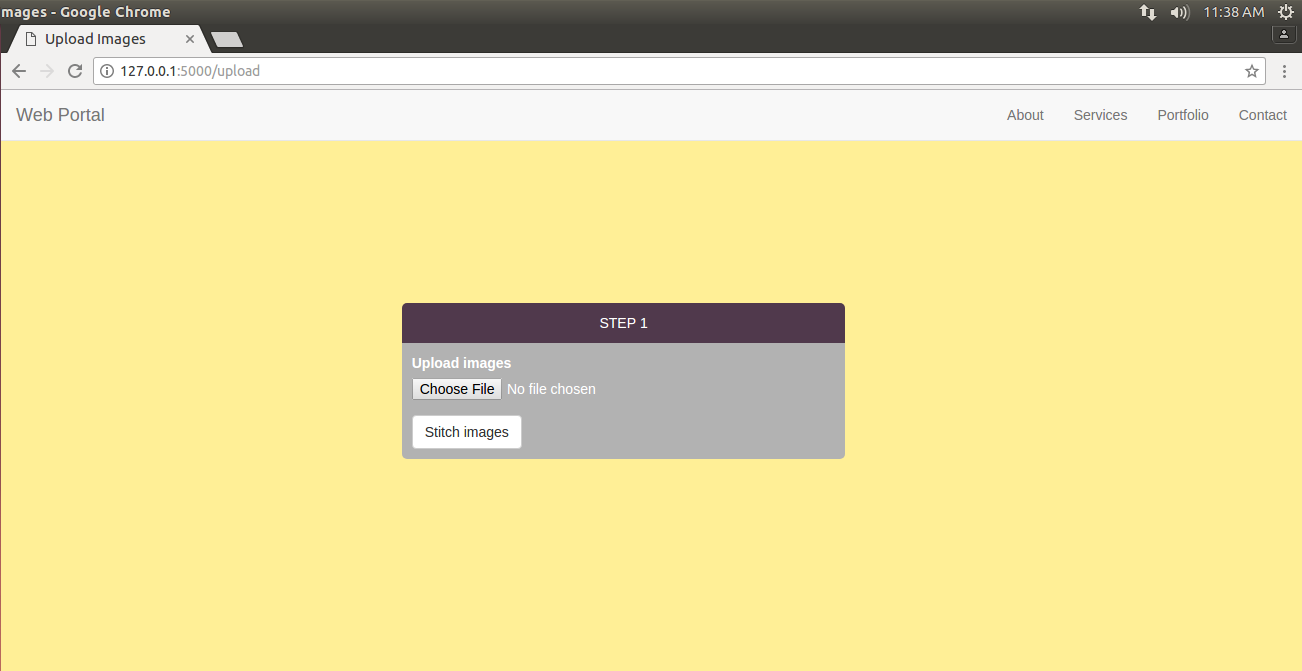
\includegraphics[width=1\linewidth]{fin_img_15}
	\centering
	\caption{\label{fig: res-1}Image upload screen}
\end{figure}
\begin{figure}[h]
	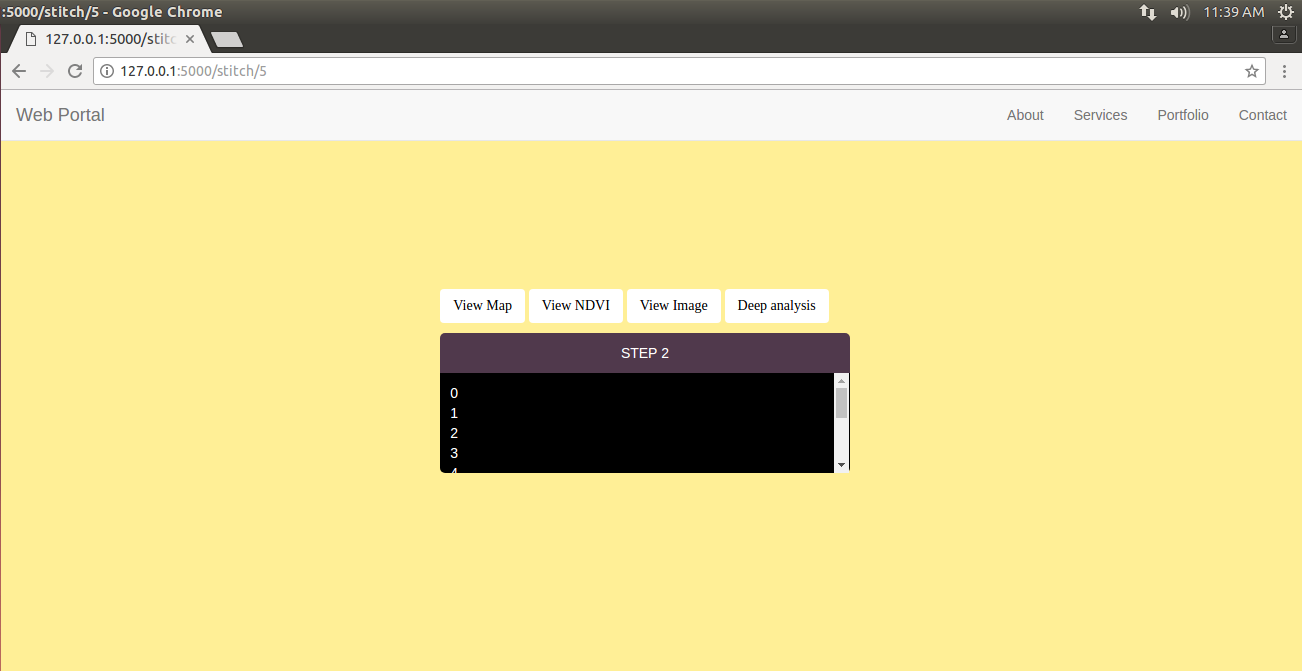
\includegraphics[width=1\linewidth]{fin_img_16}
	\centering
	\caption{\label{fig: res-2}Dashboard for Image analysis}
\end{figure}


\subsection{Dataset for Image Stitching and NDVI Analysis}

We worked upon hyperspectral images taken from drone at Hayes Township Farm, Harrison, Michigan, USA.

Figure~\ref{fig: hyp_1}, ~\ref{fig: hyp_2} and ~\ref{fig: hyp_3} shows the hyperspectral images taken from drone. (Courtesy:6omvi.org).

Figure ~\ref{fig: hyp_4} shows the image of Hayes Township Farm, Harrison, Michigan, USA


\begin{figure}[!h]
	\hfill
	\subfigure[]{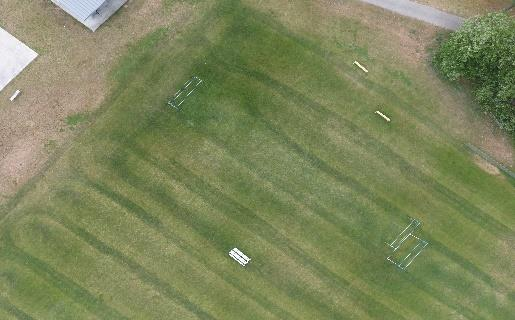
\includegraphics[width=0.48\linewidth]{fin_img_2}}
	\hfill
	\subfigure[]{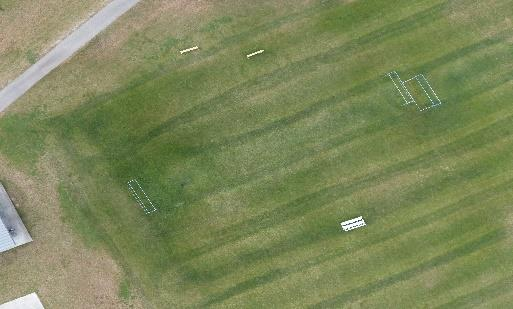
\includegraphics[width=0.48\linewidth]{fin_img_3}}
	\hfill
	\caption{\label{fig: hyp_1}Hyperspectral images taken from drone (Courtesy:6omvi.org)}
\end{figure}


\begin{figure}[!h]
	\hfill
	\subfigure[]{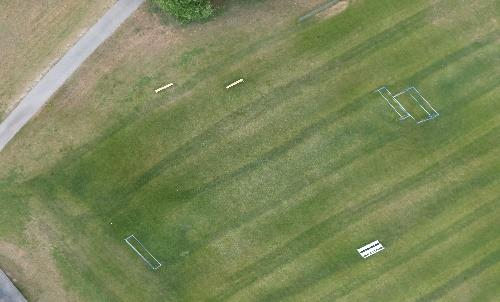
\includegraphics[width=0.48\linewidth]{fin_img_4}}
	\hfill
	\subfigure[]{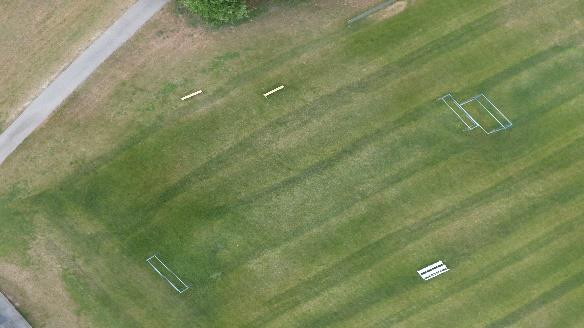
\includegraphics[width=0.48\linewidth]{fin_img_5}}
	\hfill
	\caption{\label{fig: hyp_2}Hyperspectral images taken from drone (Courtesy:6omvi.org)}
\end{figure}

\begin{figure}[!h]
	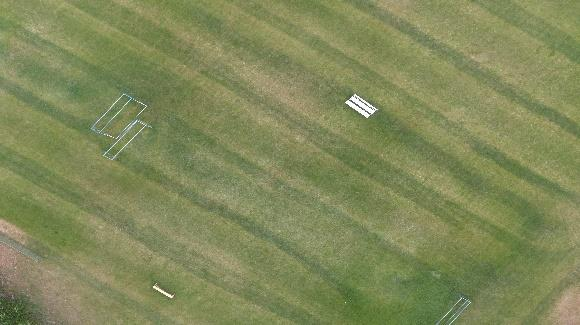
\includegraphics[width=0.5\linewidth]{fin_img_6}
	\centering
	\caption{\label{fig: hyp_3}Hyperspectral image taken from drone (Courtesy:6omvi.org)}
\end{figure}

\begin{figure}[h]
	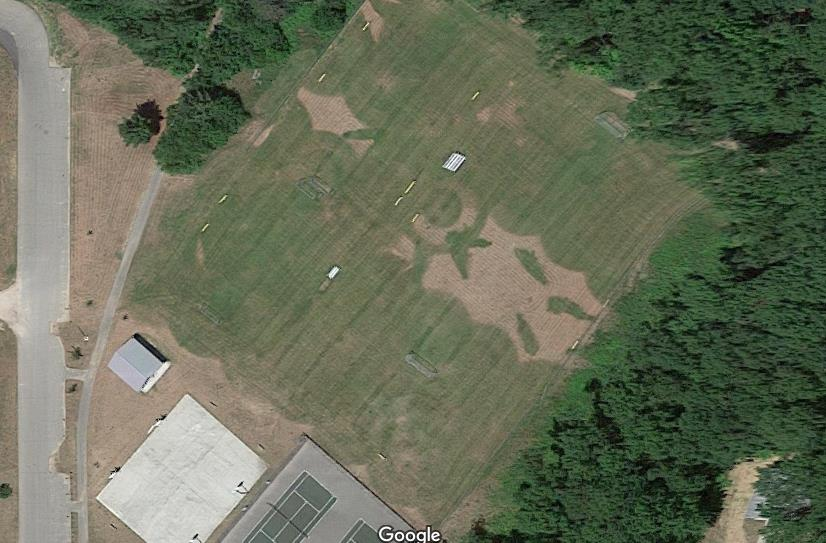
\includegraphics[width=1.0\linewidth]{fin_img_7}
	\centering
	\caption{\label{fig: hyp_4}Hayes Township Farm,Harrison,Michigan,USA.}
\end{figure}

\subsection{Image Stitching}
Image stitching is done using OpenDroneMap (ODM) library which requires 60\% overlay between input images for accurate stitching. ODM generates a stitched image in .TIF and .PNG format which can be viewed on portal by clicking on View Image button as shown in Fig.~\ref{fig: res-3}.

\begin{figure}[h]
	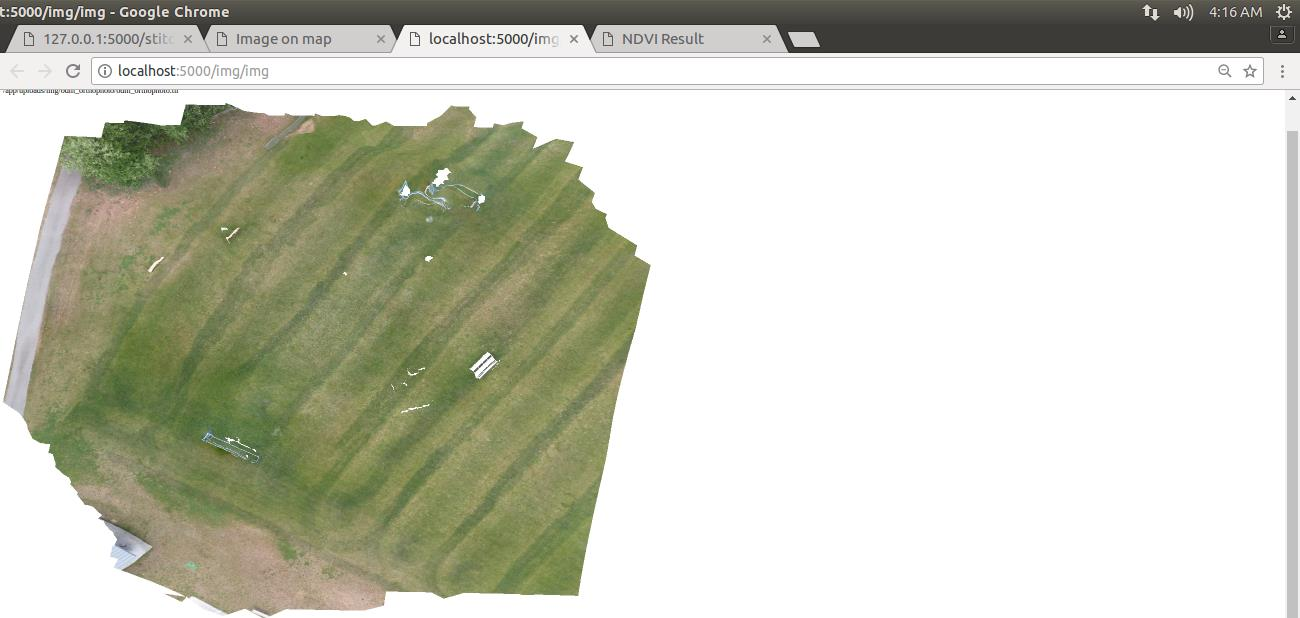
\includegraphics[width=1\linewidth]{fin_img_17}
	\centering
	\caption{\label{fig: res-3}Stitched Image output}
\end{figure}

\subsection{NDVI Analysis}

In our application we calculated NDVI using QGIS (Quantum GIS) python programing language APIs. We use QgsRasterLayer class that provides QGIS with the ability to render raster (image) datasets onto the map canvas. From loaded raster we are extracting IR and Red bands for NDVI calculation. QgsRasterCalculator (expression, output file, ``GTiff'', extent, width, height, entries) class generates NDVI image with the help of QgsRasterCalculator .processCalculation () method. View NDVI button calculates the NDVI of the stitched image as shown in Fig.~\ref{fig: stitching}

\begin{figure}[h]
	\hfill
	\subfigure[]{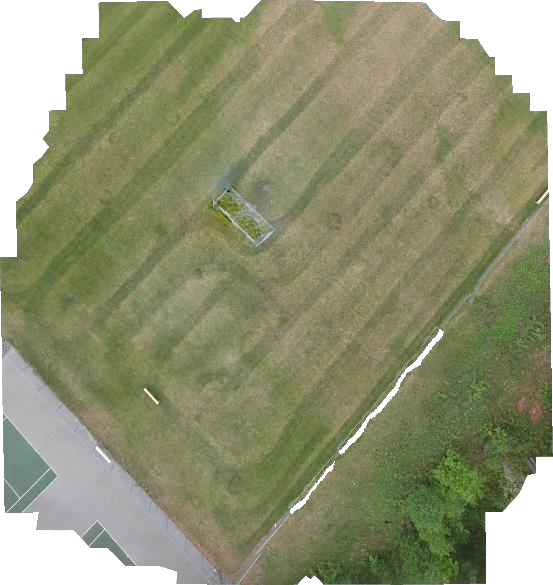
\includegraphics[width=0.48\linewidth]{fin_img_9}}
	\hfill
	\subfigure[]{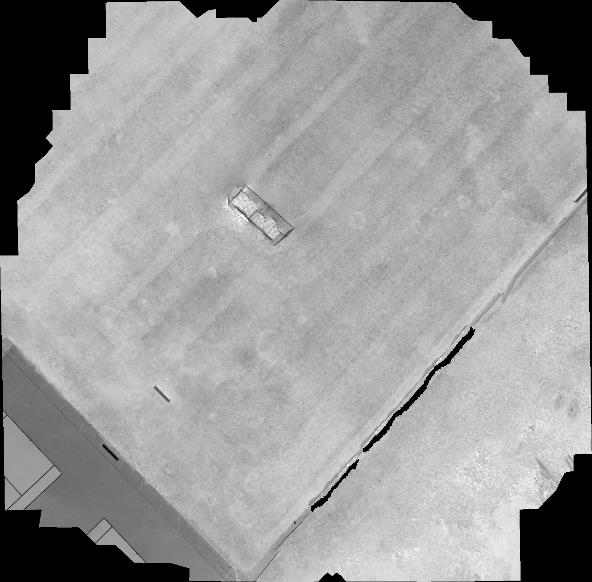
\includegraphics[width=0.48\linewidth]{fin_img_10}}
	\hfill
	\caption{\label{fig: stitching}\textbf{(a)} Input stitched image \& \textbf{(b)} NDVI output Image}
\end{figure}

\subsection{Clustering using K-Means}

We clustered the data into k = 4 classes depending upon the range of NDVI values as given by . This clustered data is used to train the SoftMax regression model.


\subsection{SoftMax Regression Model}

We built a softmax regression model using Google’s tensorflow and trained it upon the clustered dataset generated from above step. With 80\% training and 20\% test data we achieved an accuracy of about 70\%. This can be improved once we have better labelled dataset. The layered structure of the built model as visualized in TensorBoard is shown in Fig.~\ref{fig: softmax regression}

\begin{figure}[t]
	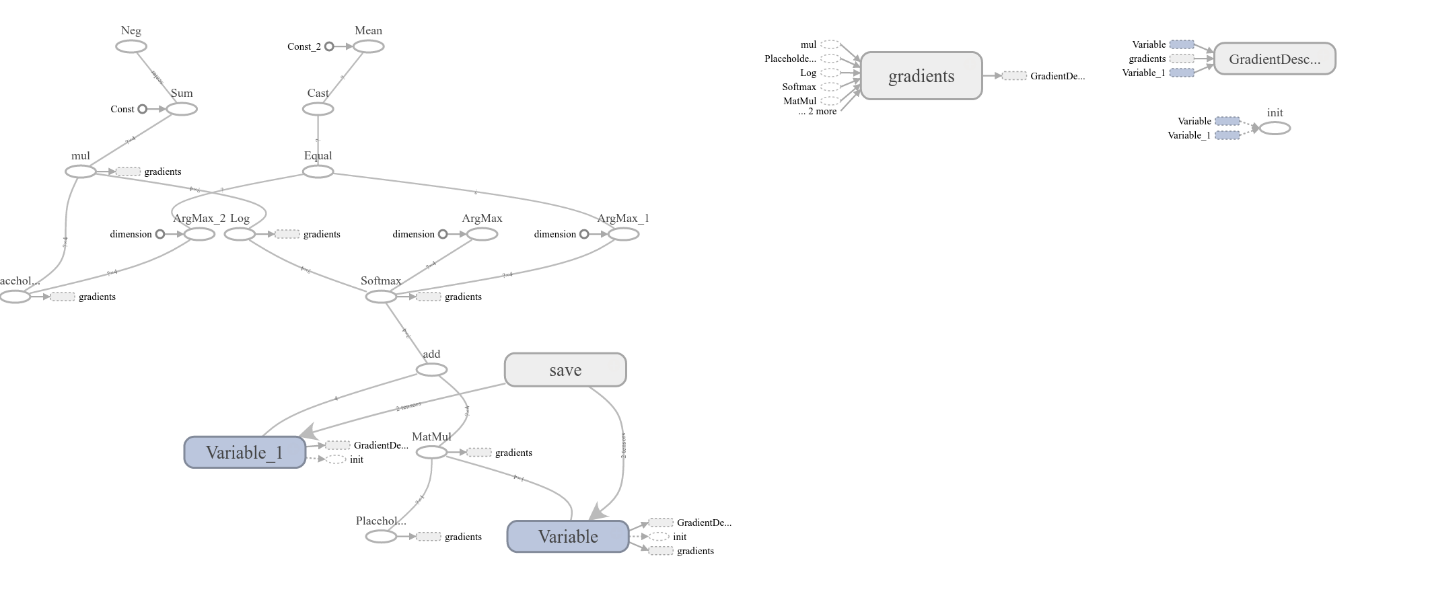
\includegraphics[width=1.0\linewidth]{fin_img_12}
	\centering
	\caption{\label{fig: softmax regression}Softmax Regression Model(Visualized in Tensorboard)}
\end{figure}

\textbf{Analysis 1 Tab}: Clicking on this button evaluates the newly created NDVI image via the Softmax Model to divide the input image into different colour coded regions as shown in Fig.~\ref{fig: res-4}

\begin{figure}[h]
	\hfill
	\subfigure[]{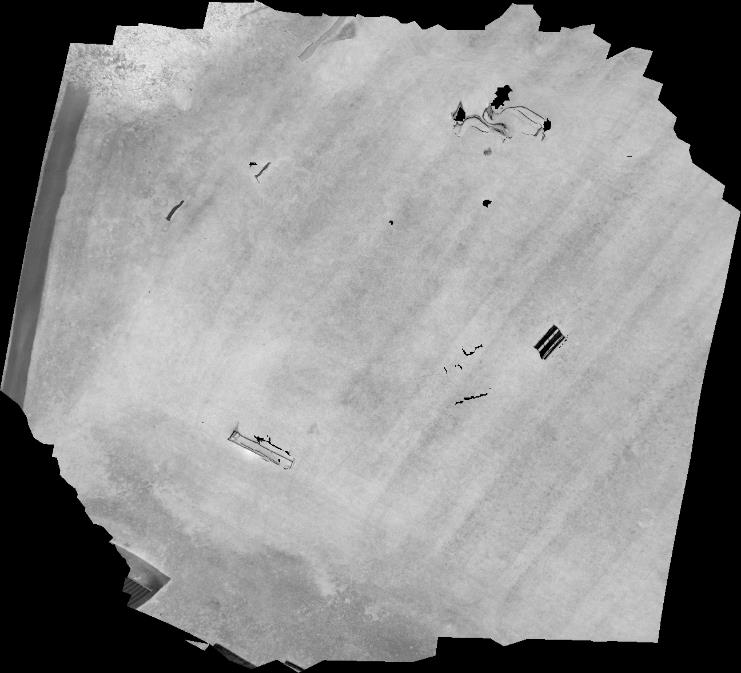
\includegraphics[width=0.48\linewidth]{fin_img_18}}
	\hfill
	\subfigure[]{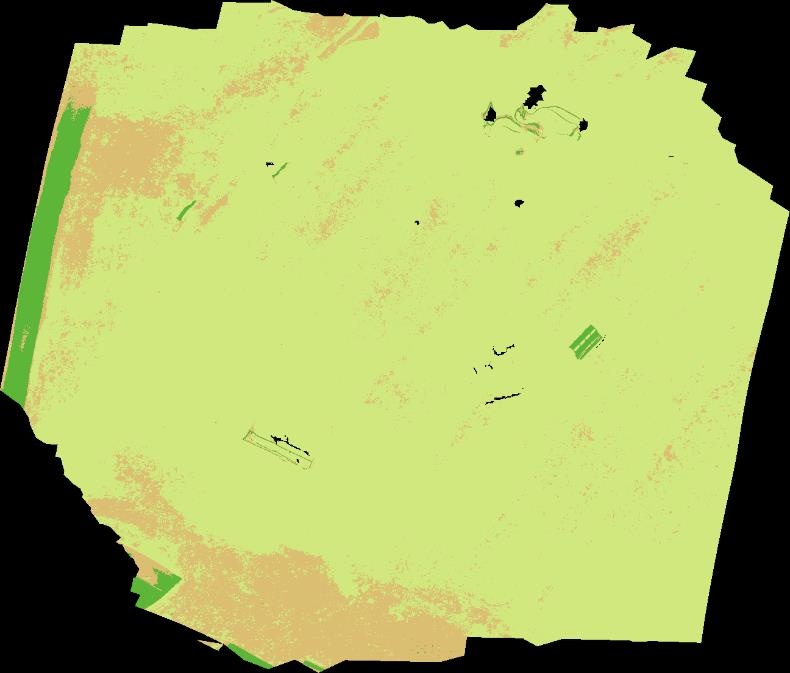
\includegraphics[width=0.48\linewidth]{fin_img_19}}
	\hfill
	\caption{\label{fig: res-4}\textbf{(a)} Stitched image \& \textbf{(b)} Colour coded regions}
\end{figure}


Finally the image of the farm is overlaid over the Google Maps as shown in Fig.~\ref{fig: res-5}

\begin{figure}[h]
	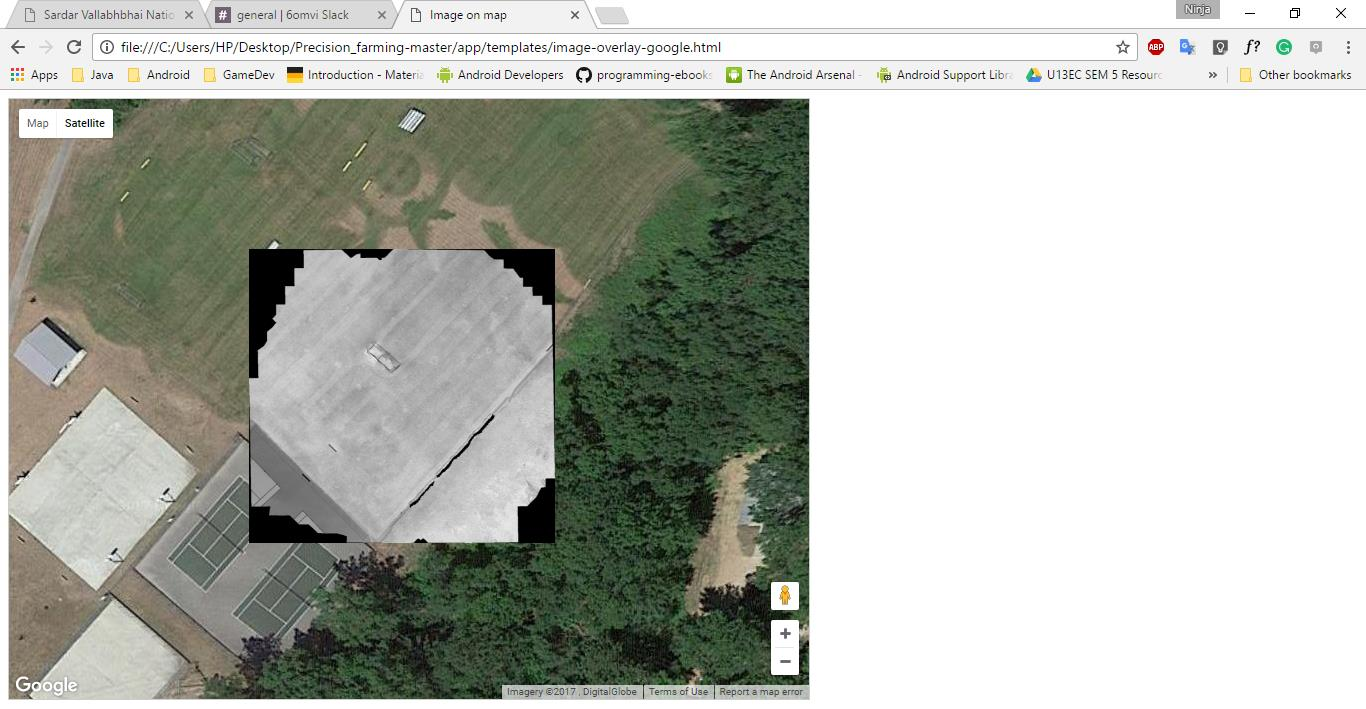
\includegraphics[width=1\linewidth]{fin_img_20}
	\centering
	\caption{\label{fig: res-5}NDVI analysed image overlaid on Google Map}
\end{figure}



\subsection{Dataset for Deep Learning}

We used a public dataset~\cite{PlantVil94:online} of 54,306 images of diseased and healthy plant leaves collected under controlled conditions to identify 14 crop species and 26 diseases (or absence thereof).An example of leaf images form the PlantVillage dataset, representing 38 crop-disease pair is hsown in Fig.~\ref{fig: dataset_image}.

\begin{figure}[!h]
	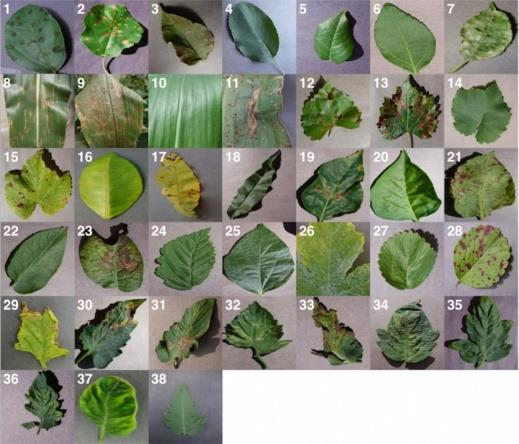
\includegraphics[width=1\linewidth]{fin_img_1}
	\centering
	\caption{\label{fig: dataset_image}Example of leaf images from the PlantVillage dataset, representing every crop-disease pair used \textbf{(1)} Apple Scab, \textit{Venturia inaequalis} \textbf{(2)} Apple Black Rot, \textit{Botryosphaeria obtusa} \textbf{(3)} Apple Cedar Rust,  \textit{Gymnosporangium juniperi-virginianae} \textbf{(4)} Apple healthy \textbf{(5)} Blueberry healthy \textbf{(6)} Cherry healthy \textbf{(7)} Cherry Powdery Mildew, \textit{Podoshaera clandestine} \textbf{(8)} Corn Gray Leaf Spot, \textit{Cercospora zeae-maydis} \textbf{(9)} Corn Common Rust, \textit{Puccinia sorghi} \textbf{(10)} Corn healthy \textbf{(11)} Corn Northern Leaf Blight, \textit{Exserohilum turcicum} \textbf{(12)} Grape Black Rot, \textit{Guignardia bidwellii}, \textbf{(13)} Grape Black Measles (Esca), \textit{Phaeomoniella aleophilum, Phaeomoniella chlamydospora} \textbf{(14)} Grape Healthy \textbf{(15)} Grape Leaf Blight, \textit{Pseudocercospora vitis} \textbf{(16)} Orange Huanglongbing (Citrus Greening), \textit{Candidatus Liberibacter spp.} \textbf{(17)} Peach Bacterial Spot, \textit{Xanthomonas campestris} \textbf{(18)} Peach healthy \textbf{(19)} Bell Pepper Bacterial Spot, \textit{Xanthomonas campestris} \textbf{(20)} Bell Pepper healthy \textbf{(21)} Potato Early Blight, \textit{Alternaria solani} \textbf{(22)} Potato healthy \textbf{(23)} Potato Late Blight, \textit{Phytophthora infestans} \textbf{(24)} Raspberry healthy \textbf{(25)} Soybean healthy \textbf{(26)} Squash Powdery Mildew, \textit{Erysiphe cichoracearum} \textbf{(27)} Strawberry Healthy \textbf{(28)} Strawberry Leaf Scorch, \textit{Diplocarpon earlianum} \textbf{(29)} Tomato Bacterial Spot, \textit{Xanthomonas campestris pv. vesicatoria} \textbf{(30)} Tomato Early Blight, \textit{Alternaria solani} \textbf{(31)} Tomato Late Blight, \textit{Phytophthora infestans} \textbf{(32)} Tomato Leaf Mold, \textit{Passalora fulva} \textbf{(33)} Tomato Septoria Leaf Spot, \textit{Septoria lycopersici} \textbf{(34)} Tomato Two Spotted Spider Mite, \textit{Tetranychus urticae} \textbf{(35)} Tomato Target Spot, \textit{Corynespora cassiicola} \textbf{(36)} Tomato Mosaic Virus \textbf{(37)} Tomato Yellow Leaf Curl Virus \textbf{(38)} Tomato healthy.}
\end{figure}


\subsection{Crop Disease Prediction Using Deep Learning}

Using the deep convolutional neural network architecture, we trained the inception V-3 model on images of plant leaves with the goal of classifying both crop species and the presence and identity of disease on images that the model had not seen before. The images were resized to 256x256 pixels as required by the inception model. Within the PlantVillage data set of 54,306 images containing 38 classes of 14 crop species and 26 diseases (or absence thereof), and with 70\% training while 30\% validation datasets this goal has been achieved as demonstrated by the top accuracy of 99\% upon training till 3900 steps for 23 hours on 32GB RAM CPU with 8GB of NVIDIA GeForce 980M GTX graphics card. Thus, without any feature engineering, the model correctly classifies crop and disease from 38 possible classes in 990 out of 1000 images. Importantly, while the training of the model takes a lot of time (multiple hours on a high performance GPU cluster computer), the classification itself is very fast (less than a second on a CPU), and can thus easily be implemented on a smartphone.


\subsubsection{Limitations}
However, this approach helps the farmers to get prescription of the crop problems, there are certain limitations to it. In this experiment we are currently constrained to  the classification of single leaves, facing up, on a homogeneous background. While these are straightforward conditions, a real world application should be able to classify images of a disease as it presents itself directly on the plant. Indeed, many diseases don’t present themselves on the upper side of leaves  only (or at all), but on many different parts of the plant. Thus, new image collection efforts should try to obtain images from many different perspectives, and ideally from settings that are as realistic as possible. This way we can get better accuracies in practical problems.

\textbf{Analysis Tab 2}: Clicking on this button on the portal asks the user to upload an image of the crops (taken by smartphone) which is evaluated against the trained inception v-3 model.


Example input image as shown in Fig.~\ref{fig: res-6} gives the output:

\begin{figure}[!h]
	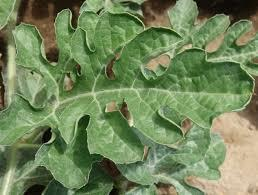
\includegraphics[width=0.5\linewidth]{fin_img_21}
	\centering
	\caption{\label{fig: res-6}Input image of crop}
\end{figure}

\textbf{Class 12: Grape Black Rot, \textit{Guignardia bidwellii} (crop-disease pair)}.

\textbf{Cause:} “Grape black rot is a fungal disease caused by an ascomycetous fungus, \textit{Guignardia bidwellii}, that attacks grape vines during hot and humid weather”

\textbf{Control:} A mixture of cultural and chemical control practices can manage grape black rot disease caused by Guignardia bidwellii. Cultural control aspects involve the basics in plant care and field sanitation as well as clean-up after an infectious outbreak. Chemical control has a large influence to eliminate disease.

A similar workflow in Android Application is shown in Fig.~\ref{fig: scr1andscr2} and Fig.~\ref{fig: scr3andscr4}.

\begin{figure}[!h]
	\hfill
	\subfigure[]{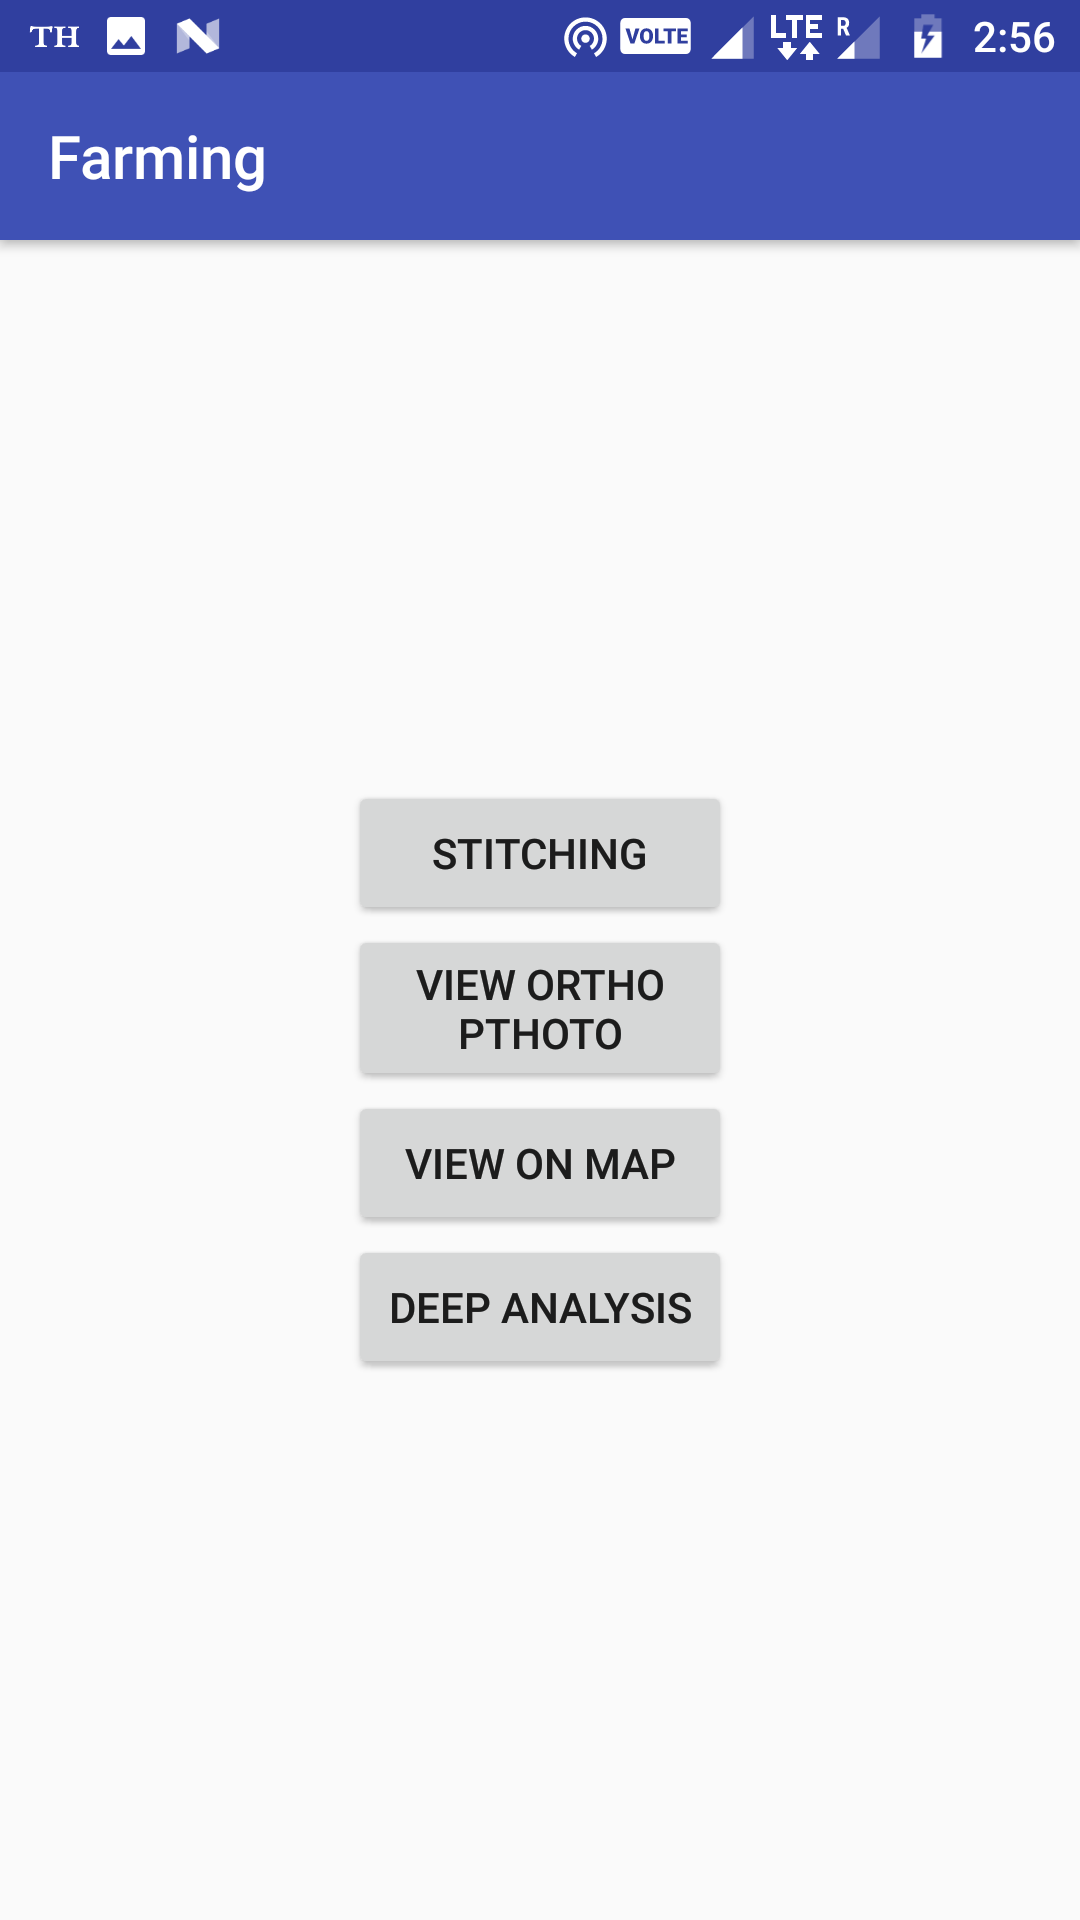
\includegraphics[height=0.48\linewidth]{scr-4}}
	\hfill
	\subfigure[]{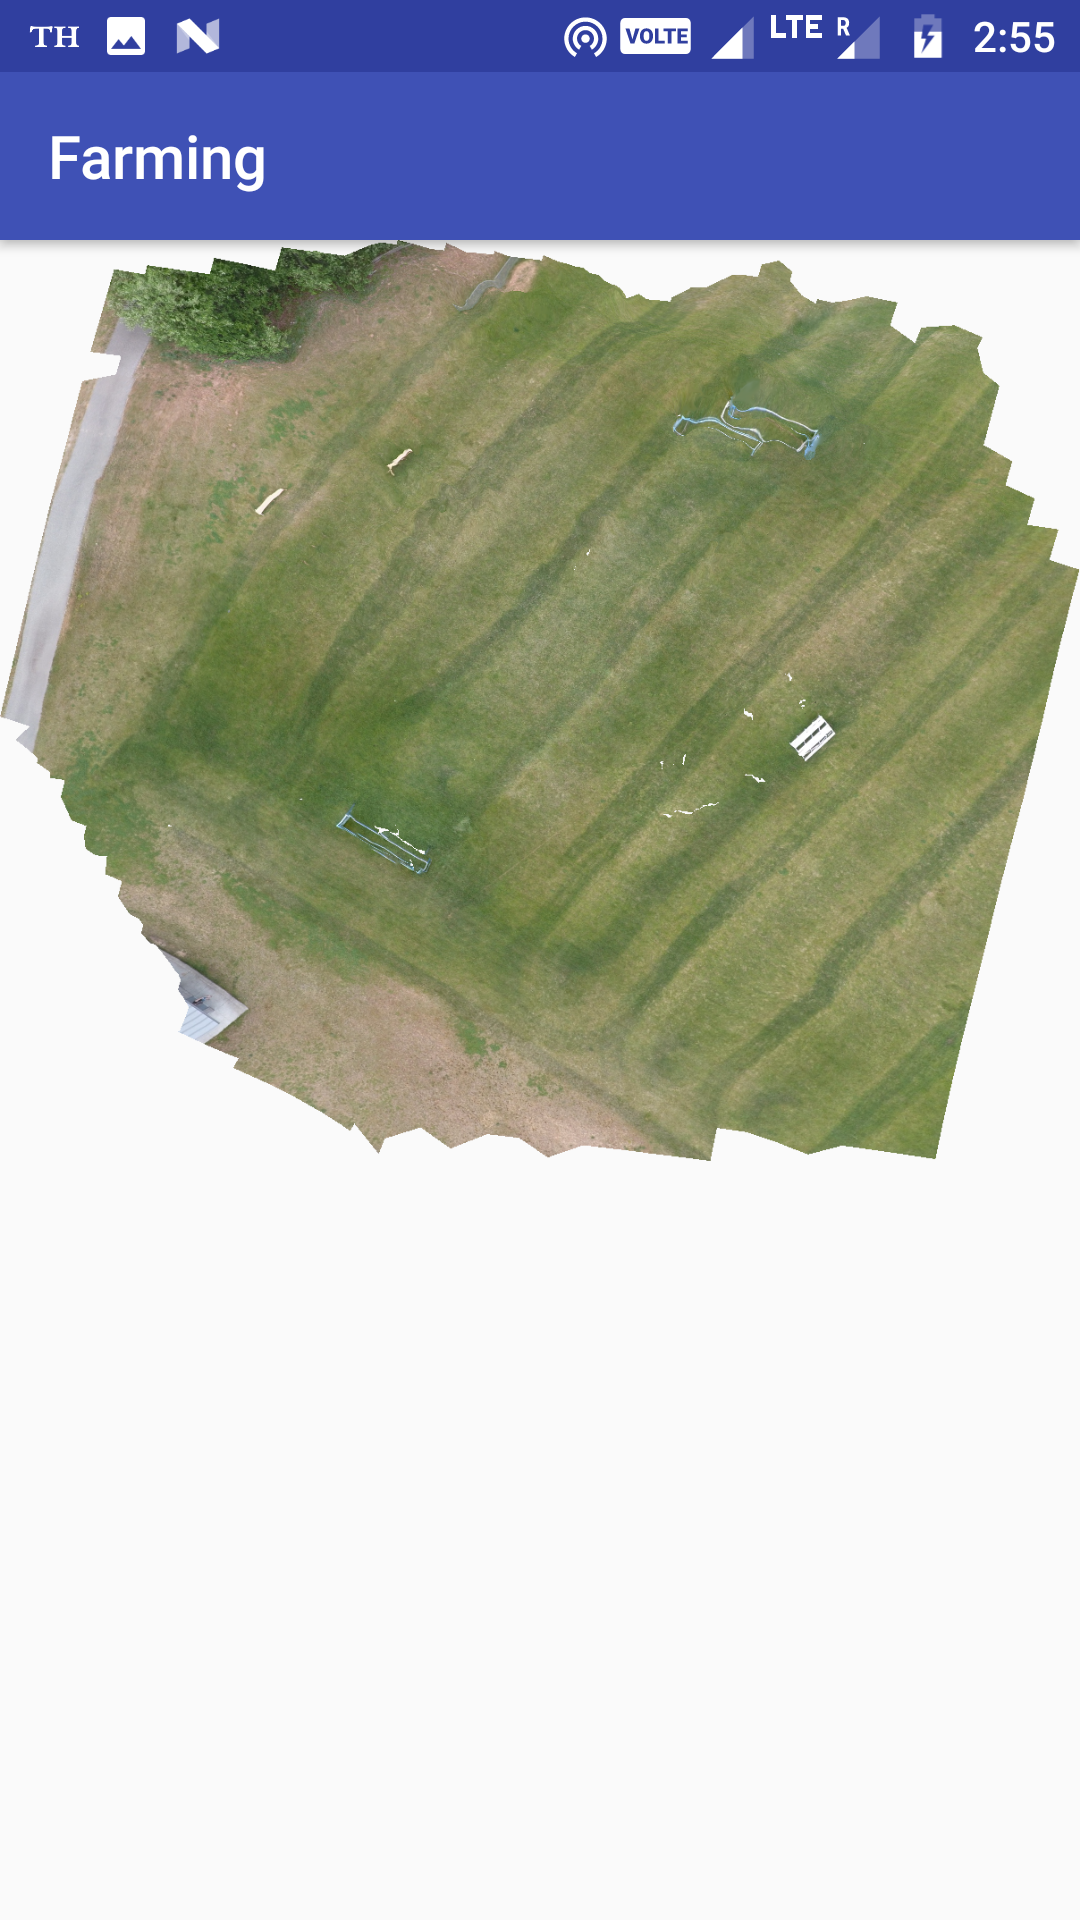
\includegraphics[height=0.48\linewidth]{scr-3}}
	\hfill
	\caption{\label{fig: scr3andscr4}Fig.~\ref{fig: scr3andscr4}(a) describes Home Screen of Android Application. Fig.~\ref{fig: scr3andscr4}(b) shows Stitched image output}
\end{figure}


\begin{figure}[!h]
	\hfill
	\subfigure[]{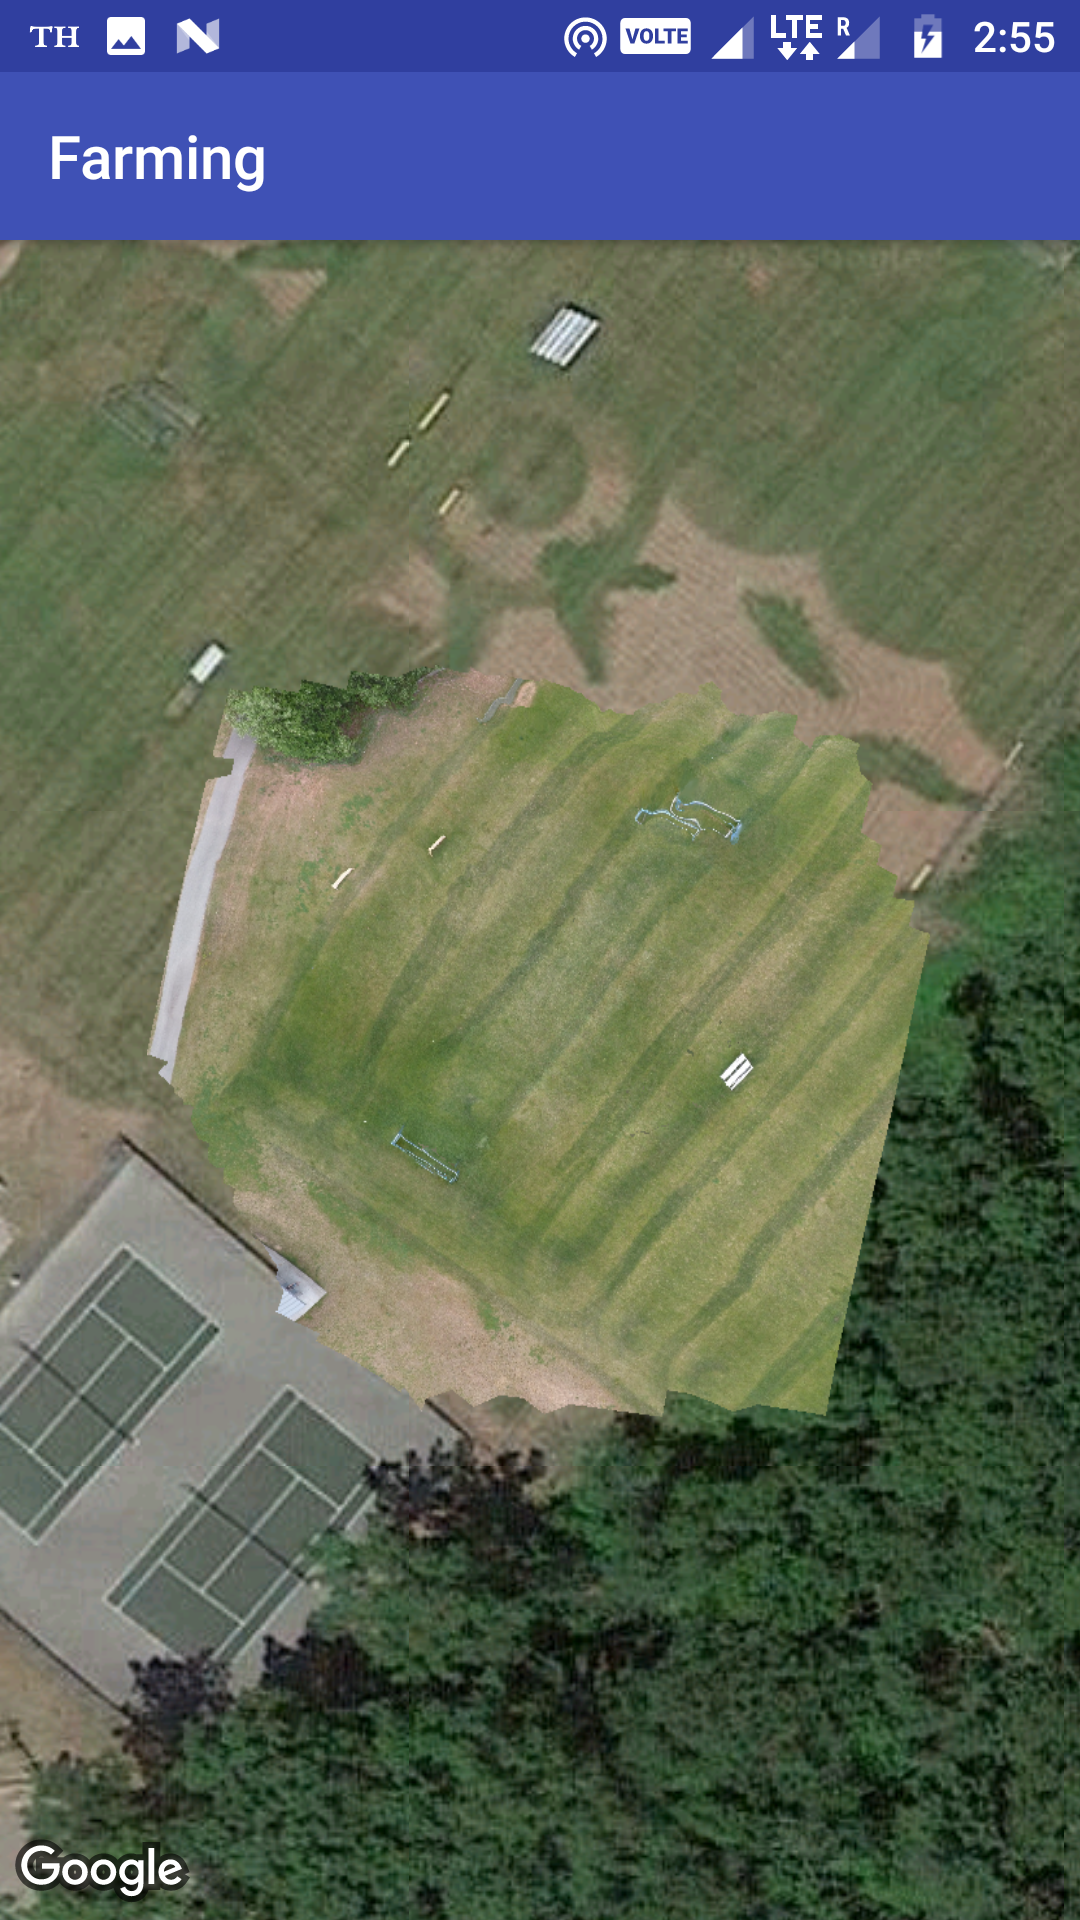
\includegraphics[height=0.48\linewidth]{scr-2}}
	\hfill
	\subfigure[]{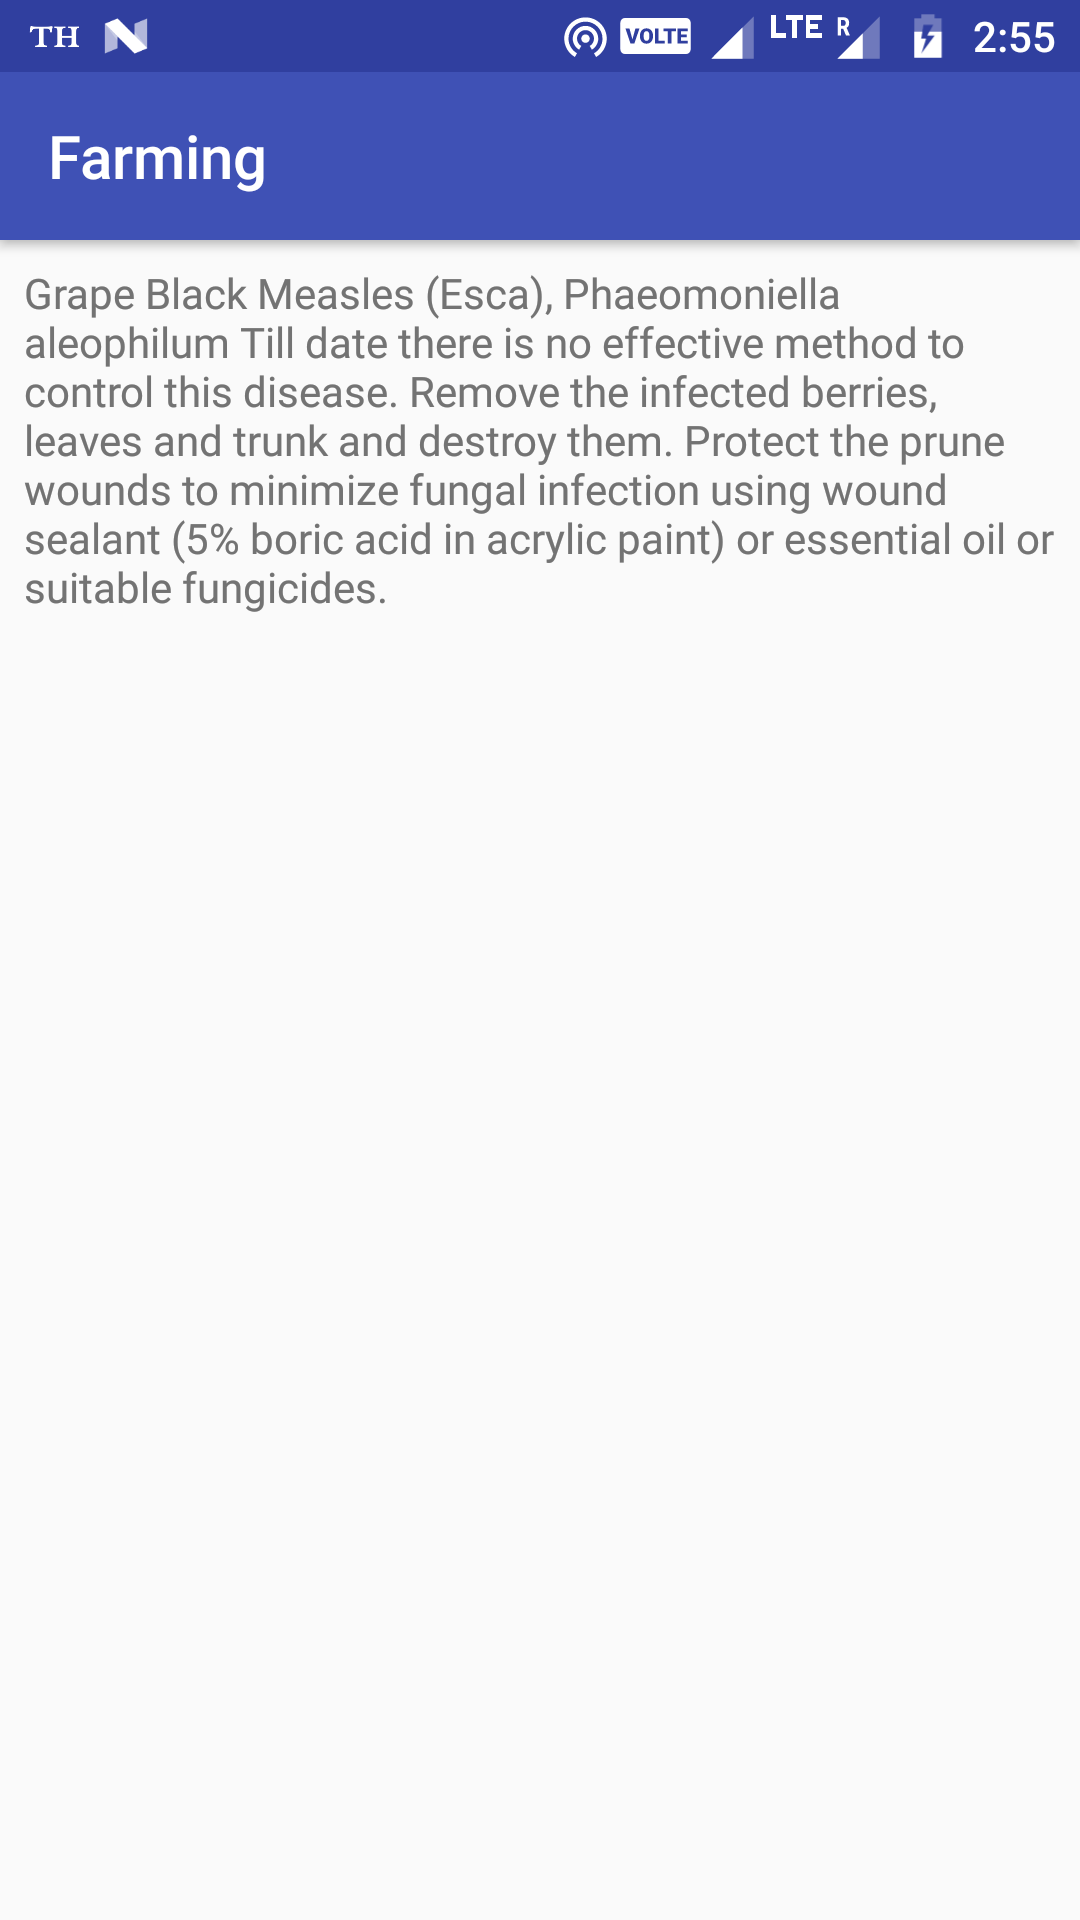
\includegraphics[height=0.48\linewidth]{scr-1}}
	\hfill
	\caption{\label{fig: scr1andscr2}Fig.~\ref{fig: scr1andscr2}(a) describes overlay of stitched image on Google Maps. Fig.~\ref{fig: scr1andscr2} describes prescription of crops in critical areas of the farm.}
\end{figure}